\documentclass[12pt]{report}
\usepackage{suthesis}

% -- Imports --
% (general libraries)
\usepackage{times,latexsym,amsfonts,amssymb,amsmath,graphicx,url,bbm,rotating}
\usepackage{multirow,hhline,stmaryrd,bussproofs,mathtools,siunitx}
\usepackage{booktabs,xcolor,csquotes,calligra}
\usepackage{mhchem}
% (custom libraries)
\usepackage{afterpage}
\usepackage{longtable}
\usepackage{fitch}
% (inline references)
\usepackage{natbib}
\usepackage{tabularx}
\usepackage[hidelinks]{hyperref}
\hypersetup{
    colorlinks=true,
    citecolor=magenta,
    linkcolor=.,
    urlcolor=blue
}

\usepackage{epigraph}
\renewcommand{\epigraphsize}{\normalsize}
\setlength{\epigraphwidth}{0.9\textwidth}

% (tikz)
\usepackage{soul}
\definecolor{light-yellow}{RGB}{255, 255, 153}
\sethlcolor{light-yellow}
\usepackage{tikz}
\usepackage{tikz-dependency,pifont}
\usetikzlibrary{shapes.arrows,chains,positioning,automata,trees,calc}
\usetikzlibrary{patterns,matrix}
\usetikzlibrary{decorations.pathmorphing,decorations.markings}
% (print algorithms)
\usepackage[ruled,lined,linesnumbered]{algorithm2e}
% (custom)
% version 1.2 05/21/08
\newcommand\sa{\ensuremath{\mathcal{a}}}
\newcommand\sd{\ensuremath{\mathcal{d}}}
\newcommand\se{\ensuremath{\mathcal{e}}}
\newcommand\sg{\ensuremath{\mathcal{g}}}
\newcommand\sh{\ensuremath{\mathcal{h}}}
\newcommand\seye{\ensuremath{\mathcal{i}}}
\newcommand\sj{\ensuremath{\mathcal{j}}}
\newcommand\sk{\ensuremath{\mathcal{k}}}
\newcommand\sm{\ensuremath{\mathcal{m}}}
\newcommand\sn{\ensuremath{\mathcal{n}}}
\newcommand\sq{\ensuremath{\mathcal{q}}}
\newcommand\sr{\ensuremath{\mathcal{r}}}
\newcommand\su{\ensuremath{\mathcal{u}}}
\newcommand\sv{\ensuremath{\mathcal{v}}}
\newcommand\sw{\ensuremath{\mathcal{w}}}
\newcommand\sx{\ensuremath{\mathcal{x}}}
\newcommand\sy{\ensuremath{\mathcal{y}}}
\newcommand\sz{\ensuremath{\mathcal{z}}}
\newcommand\sA{\ensuremath{\mathcal{A}}}
\newcommand\sB{\ensuremath{\mathcal{B}}}
\newcommand\sC{\ensuremath{\mathcal{C}}}
\newcommand\sD{\ensuremath{\mathcal{D}}}
\newcommand\sE{\ensuremath{\mathcal{E}}}
\newcommand\sF{\ensuremath{\mathcal{F}}}
\newcommand\sG{\ensuremath{\mathcal{G}}}
\newcommand\sH{\ensuremath{\mathcal{H}}}
\newcommand\sI{\ensuremath{\mathcal{I}}}
\newcommand\sJ{\ensuremath{\mathcal{J}}}
\newcommand\sK{\ensuremath{\mathcal{K}}}
\newcommand\sL{\ensuremath{\mathcal{L}}}
\newcommand\sM{\ensuremath{\mathcal{M}}}
\newcommand\sN{\ensuremath{\mathcal{N}}}
\newcommand\sO{\ensuremath{\mathcal{O}}}
\newcommand\sP{\ensuremath{\mathcal{P}}}
\newcommand\sQ{\ensuremath{\mathcal{Q}}}
\newcommand\sR{\ensuremath{\mathcal{R}}}
\newcommand\sS{\ensuremath{\mathcal{S}}}
\newcommand\sT{\ensuremath{\mathcal{T}}}
\newcommand\sU{\ensuremath{\mathcal{U}}}
\newcommand\sV{\ensuremath{\mathcal{V}}}
\newcommand\sW{\ensuremath{\mathcal{W}}}
\newcommand\sX{\ensuremath{\mathcal{X}}}
\newcommand\sY{\ensuremath{\mathcal{Y}}}
\newcommand\sZ{\ensuremath{\mathcal{Z}}}
\newcommand\ba{\ensuremath{\mathbf{a}}}
\newcommand\bb{\ensuremath{\mathbf{b}}}
\newcommand\bc{\ensuremath{\mathbf{c}}}
\newcommand\bd{\ensuremath{\mathbf{d}}}
\newcommand\be{\ensuremath{\mathbf{e}}}
\newcommand\bef{\ensuremath{\mathbf{f}}}
\newcommand\bg{\ensuremath{\mathbf{g}}}
\newcommand\bh{\ensuremath{\mathbf{h}}}
\newcommand\bi{\ensuremath{\mathbf{i}}}
\newcommand\bj{\ensuremath{\mathbf{j}}}
\newcommand\bk{\ensuremath{\mathbf{k}}}
\newcommand\bl{\ensuremath{\mathbf{l}}}
\newcommand\bn{\ensuremath{\mathbf{n}}}
\newcommand\bo{\ensuremath{\mathbf{o}}}
\newcommand\bp{\ensuremath{\mathbf{p}}}
\newcommand\bq{\ensuremath{\mathbf{q}}}
\newcommand\br{\ensuremath{\mathbf{r}}}
\newcommand\bs{\ensuremath{\mathbf{s}}}
\newcommand\bt{\ensuremath{\mathbf{t}}}
\newcommand\bu{\ensuremath{\mathbf{u}}}
\newcommand\bv{\ensuremath{\mathbf{v}}}
\newcommand\bw{\ensuremath{\mathbf{w}}}
\newcommand\bx{\ensuremath{\mathbf{x}}}
\newcommand\by{\ensuremath{\mathbf{y}}}
\newcommand\bz{\ensuremath{\mathbf{z}}}
\newcommand\bA{\ensuremath{\mathbf{A}}}
\newcommand\bB{\ensuremath{\mathbf{B}}}
\newcommand\bC{\ensuremath{\mathbf{C}}}
\newcommand\bD{\ensuremath{\mathbf{D}}}
\newcommand\bE{\ensuremath{\mathbf{E}}}
\newcommand\bF{\ensuremath{\mathbf{F}}}
\newcommand\bG{\ensuremath{\mathbf{G}}}
\newcommand\bH{\ensuremath{\mathbf{H}}}
\newcommand\bI{\ensuremath{\mathbf{I}}}
\newcommand\bJ{\ensuremath{\mathbf{J}}}
\newcommand\bK{\ensuremath{\mathbf{K}}}
\newcommand\bL{\ensuremath{\mathbf{L}}}
\newcommand\bM{\ensuremath{\mathbf{M}}}
\newcommand\bN{\ensuremath{\mathbf{N}}}
\newcommand\bO{\ensuremath{\mathbf{O}}}
\newcommand\bP{\ensuremath{\mathbf{P}}}
\newcommand\bQ{\ensuremath{\mathbf{Q}}}
\newcommand\bR{\ensuremath{\mathbf{R}}}
\newcommand\bS{\ensuremath{\mathbf{S}}}
\newcommand\bT{\ensuremath{\mathbf{T}}}
\newcommand\bU{\ensuremath{\mathbf{U}}}
\newcommand\bV{\ensuremath{\mathbf{V}}}
\newcommand\bW{\ensuremath{\mathbf{W}}}
\newcommand\bX{\ensuremath{\mathbf{X}}}
\newcommand\bY{\ensuremath{\mathbf{Y}}}
\newcommand\bZ{\ensuremath{\mathbf{Z}}}
\newcommand\Ba{\ensuremath{\mathbb{a}}}
\newcommand\Bb{\ensuremath{\mathbb{b}}}
\newcommand\Bc{\ensuremath{\mathbb{c}}}
\newcommand\Bd{\ensuremath{\mathbb{d}}}
\newcommand\Be{\ensuremath{\mathbb{e}}}
\newcommand\Bf{\ensuremath{\mathbb{f}}}
\newcommand\Bg{\ensuremath{\mathbb{g}}}
\newcommand\Bh{\ensuremath{\mathbb{h}}}
\newcommand\Bi{\ensuremath{\mathbb{i}}}
\newcommand\Bj{\ensuremath{\mathbb{j}}}
\newcommand\Bk{\ensuremath{\mathbb{k}}}
\newcommand\Bl{\ensuremath{\mathbb{l}}}
\newcommand\Bm{\ensuremath{\mathbb{m}}}
\newcommand\Bn{\ensuremath{\mathbb{n}}}
\newcommand\Bo{\ensuremath{\mathbb{o}}}
\newcommand\Bp{\ensuremath{\mathbb{p}}}
\newcommand\Bq{\ensuremath{\mathbb{q}}}
\newcommand\Br{\ensuremath{\mathbb{r}}}
\newcommand\Bs{\ensuremath{\mathbb{s}}}
\newcommand\Bt{\ensuremath{\mathbb{t}}}
\newcommand\Bu{\ensuremath{\mathbb{u}}}
\newcommand\Bv{\ensuremath{\mathbb{v}}}
\newcommand\Bw{\ensuremath{\mathbb{w}}}
\newcommand\Bx{\ensuremath{\mathbb{x}}}
\newcommand\By{\ensuremath{\mathbb{y}}}
\newcommand\Bz{\ensuremath{\mathbb{z}}}
\newcommand\BA{\ensuremath{\mathbb{A}}}
\newcommand\BB{\ensuremath{\mathbb{B}}}
\newcommand\BC{\ensuremath{\mathbb{C}}}
\newcommand\BD{\ensuremath{\mathbb{D}}}
\newcommand\BE{\ensuremath{\mathbb{E}}}
\newcommand\BF{\ensuremath{\mathbb{F}}}
\newcommand\BG{\ensuremath{\mathbb{G}}}
\newcommand\BH{\ensuremath{\mathbb{H}}}
\newcommand\BI{\ensuremath{\mathbb{I}}}
\newcommand\BJ{\ensuremath{\mathbb{J}}}
\newcommand\BK{\ensuremath{\mathbb{K}}}
\newcommand\BL{\ensuremath{\mathbb{L}}}
\newcommand\BM{\ensuremath{\mathbb{M}}}
\newcommand\BN{\ensuremath{\mathbb{N}}}
\newcommand\BO{\ensuremath{\mathbb{O}}}
\newcommand\BP{\ensuremath{\mathbb{P}}}
\newcommand\BQ{\ensuremath{\mathbb{Q}}}
\newcommand\BR{\ensuremath{\mathbb{R}}}
\newcommand\BS{\ensuremath{\mathbb{S}}}
\newcommand\BT{\ensuremath{\mathbb{T}}}
\newcommand\BU{\ensuremath{\mathbb{U}}}
\newcommand\BV{\ensuremath{\mathbb{V}}}
\newcommand\BW{\ensuremath{\mathbb{W}}}
\newcommand\BX{\ensuremath{\mathbb{X}}}
\newcommand\BY{\ensuremath{\mathbb{Y}}}
\newcommand\BZ{\ensuremath{\mathbb{Z}}}
\newcommand\balpha{\ensuremath{\mbox{\boldmath$\alpha$}}}
\newcommand\bbeta{\ensuremath{\mbox{\boldmath$\beta$}}}
\newcommand\btheta{\ensuremath{\mbox{\boldmath$\theta$}}}
\newcommand\bphi{\ensuremath{\mbox{\boldmath$\phi$}}}
\newcommand\bpi{\ensuremath{\mbox{\boldmath$\pi$}}}
\newcommand\bpsi{\ensuremath{\mbox{\boldmath$\psi$}}}
\newcommand\bmu{\ensuremath{\mbox{\boldmath$\mu$}}}
% Basic
\newcommand\T{\text}
\newcommand\sign{\text{sign}}
\newcommand\tr{\text{tr}}
\newcommand\fig[1]{\begin{center} \includegraphics{#1} \end{center}}
\newcommand\Fig[5]{\begin{figure}[tb] \begin{center} \includegraphics[scale=#2]{#1} \end{center} \longcaption{#4}{\label{fig:#3} #5} \end{figure}}
\newcommand\FigTop[4]{\begin{figure}[t] \begin{center} \includegraphics[scale=#2]{#1} \end{center} \caption{\label{fig:#3} #4} \end{figure}}
\newcommand\FigStar[4]{\begin{figure*}[tb] \begin{center} \includegraphics[scale=#2]{#1} \end{center} \caption{\label{fig:#3} #4} \end{figure*}}
\newcommand\aside[1]{\quad\text{[#1]}}
\newcommand\homework[3]{\title{#1} \author{#2} \date{#3} \maketitle}
% Math
\newcommand\argmin{\mathop{\text{argmin}}}
\newcommand\argmax{\mathop{\text{argmax}}}
\newcommand\p[1]{\ensuremath{\left( #1 \right)}} % Parenthesis ()
\newcommand\pb[1]{\ensuremath{\left[ #1 \right]}} % []
\newcommand\pc[1]{\ensuremath{\left\{ #1 \right\}}} % {}
\newcommand\eval[2]{\ensuremath{\left. #1 \right|_{#2}}} % Evaluation
\newcommand\inv[1]{\ensuremath{\frac{1}{#1}}}
\newcommand\half{\ensuremath{\frac{1}{2}}}
\newcommand\R{\ensuremath{\mathbb{R}}} % Real numbers
\newcommand\Z{\ensuremath{\mathbb{Z}}} % Integers
\newcommand\inner[2]{\ensuremath{\left< #1, #2 \right>}} % Inner product
\newcommand\mat[2]{\ensuremath{\left(\begin{array}{#1}#2\end{array}\right)}} % Matrix
\newcommand\eqn[1]{\begin{eqnarray} #1 \end{eqnarray}} % Equation (array)
\newcommand\eqnl[2]{\begin{eqnarray} \label{eqn:#1} #2 \end{eqnarray}} % Equation (array) with label
\newcommand\eqdef{\ensuremath{\stackrel{\rm def}{=}}} % Equal by definition
%\newcommand{\1}{\mathbb{I}} % Indicator (don't use \mathbbm{1} because bbm is not TrueType though)
\newcommand{\1}{\ensuremath{\mathbbm{1}}}
\newcommand{\bone}{\mathbf{1}} % for vector one
\newcommand{\bzero}{\mathbf{0}} % for vector zero
\newcommand\refeqn[1]{(\ref{eqn:#1})}
\newcommand\refeqns[2]{(\ref{eqn:#1}) and (\ref{eqn:#2})}
\newcommand\refchp[1]{Chapter~\ref{chp:#1}}
\newcommand\refsec[1]{Section~\ref{sec:#1}}
\newcommand\refsecs[2]{Sections~\ref{sec:#1} and~\ref{sec:#2}}
\newcommand\reffig[1]{Figure~\ref{fig:#1}}
\newcommand\reffigs[2]{Figures~\ref{fig:#1} and~\ref{fig:#2}}
\newcommand\reffigss[3]{Figures~\ref{fig:#1},~\ref{fig:#2}, and~\ref{fig:#3}}
\newcommand\reffigsss[4]{Figures~\ref{fig:#1},~\ref{fig:#2},~\ref{fig:#3}, and~\ref{fig:#4}}
\newcommand\reftab[1]{Table~\ref{tab:#1}}
\newcommand\refapp[1]{Appendix~\ref{sec:#1}}
\newcommand\refthm[1]{Theorem~\ref{thm:#1}}
\newcommand\refthms[2]{Theorems~\ref{thm:#1} and~\ref{thm:#2}}
\newcommand\reflem[1]{Lemma~\ref{lem:#1}}
\newcommand\reflems[2]{Lemmas~\ref{lem:#1} and~\ref{lem:#2}}
\newcommand\refprop[1]{Proposition~\ref{prop:#1}}
\newcommand\refdef[1]{Definition~\ref{def:#1}}
\newcommand\refcor[1]{Corollary~\ref{cor:#1}}
\newcommand\refalg[1]{Algorithm~\ref{alg:#1}}

\newcommand\Chapter[2]{\chapter{#2}\label{chp:#1}}
\newcommand\Section[2]{\section{#2}\label{sec:#1}}
\newcommand\Subsection[2]{\subsection{#2}\label{sec:#1}}
\newcommand\Subsubsection[2]{\subsubsection{#2}\label{sec:#1}}
%\newtheorem{definition}{Definition}
%\newtheorem{assumption}{Assumption}
%\newtheorem{proposition}{Proposition}
%\newtheorem{theorem}{Theorem}
%\newtheorem{lemma}{Lemma}
%\newtheorem{corollary}{Corollary}
% Probability
\newcommand\cv{\ensuremath{\to}} % Convergence
\newcommand\cvL{\ensuremath{\xrightarrow{\mathcal{L}}}} % Convergence in law
\newcommand\cvd{\ensuremath{\xrightarrow{d}}} % Convergence in distribution
\newcommand\cvP{\ensuremath{\xrightarrow{P}}} % Convergence in probability
\newcommand\cvas{\ensuremath{\xrightarrow{a.s.}}} % Convergence almost surely
\newcommand\eqdistrib{\ensuremath{\stackrel{d}{=}}} % Equal in distribution
\newcommand\E[1]{\ensuremath{\mathbb{E}{\left[#1\right]}}} % Expectation
\newcommand\Ex[2]{\ensuremath{\mathbb{E}_{#1}\left[#2\right]}} % Expectation
%\newcommand\var{\ensuremath{\text{var}}} % Variance
\newcommand\cov{\ensuremath{\text{cov}}} % Covariance
\newcommand\diag{\ensuremath{\text{diag}}} % Diagnonal matrix
\newcommand\cE[2]{\ensuremath{\E \left( #1 \mid #2 \right)}} % Conditional expectation
\newcommand\KL[2]{\ensuremath{\T{KL}\left( #1 \,||\, #2 \right)}} % KL-divergence
\newcommand\D[2]{\ensuremath{\bD\left( #1 \,||\, #2 \right)}} % KL-divergence

% Utilities
\newcommand\lte{\leq}
\newcommand\gte{\geq}
\newcommand\lone[1]{\ensuremath{\|#1\|_1}}
\newcommand\ltwo[1]{\ensuremath{\|#1\|_2^2}}
\newcommand\naive{na\"{\i}ve}
\newcommand\Naive{Na\"{\i}ve}

% Debug
\usepackage{color}
\newcommand{\tred}[1]{\textcolor{red}{#1}}
\newcommand{\hly}[1]{\hl{yellow}{#1}}
% \def\todo#1{\hl{{\bf TODO:} #1}{yellow}}
\def\needcite{\hl{{$^{\tt\small[citation\ needed]}$}}{blue}}
\def\needfig{\hl{Figure X}{green}}
\def\needtab{\hl{Table Y}{green}}
\def\note#1{\hl{{\bf NOTE:} #1}{yellow}}
\def\dome{\hl{{\bf TODO:} write me!}{yellow}}

% (tweaks)
\definecolor{darkred}{rgb}{0.5451, 0.0, 0.0}
\definecolor{darkgreen}{rgb}{0.0, 0.3922, 0.0}

\def\blue#1{\textcolor{blue}{#1}}
\def\darkblue#1{\textcolor{blue}{#1}}
\def\red#1{\textcolor{red}{#1}}
\def\darkred#1{\textcolor{darkred}{#1}}
\def\green#1{\textcolor{green}{#1}}
\def\darkgreen#1{\textcolor{darkgreen}{#1}}
\def\yellow#1{\textcolor{yellow}{#1}}
\definecolor{burntorange}{HTML}{BF5700}
\def\orange#1{\textcolor{burntorange}{#1}}
\def\gray#1{\textcolor{gray}{#1}}
\def\darkgray#1{\textcolor{darkgray}{#1}}

\newcommand\sys[1]{\textsc{#1}}
\newcommand\ti[1]{\textit{#1}}
\newcommand\tf[1]{\textbf{#1}}
\newcommand\mf[1]{\mathbf{#1}}
\newcommand{\indentitem}{\setlength\itemindent{25pt}}
\newcommand{\nth}{$^{\textrm{th}}$}

\newcommand\denote[1]{\ensuremath{\llbracket\ti{#1}\rrbracket}}

\newcommand\forward{\ensuremath{\sqsubseteq}}
\newcommand\nforward{\ensuremath{\not\sqsubseteq}}
\newcommand\reverse{\ensuremath{\sqsupseteq}}
\newcommand\alternate{\ensuremath{\downharpoonleft\hspace{-1.25mm}\upharpoonright}}
\newcommand\cover{\ensuremath{\smallsmile}}
\newcommand\equivalent{\ensuremath{\equiv}}
\newcommand\negate{\ensuremath{\curlywedge}}
\newcommand\independent{\ensuremath{\#}}
\newcommand\tagUp[1]{#1\ensuremath{^\uparrow}}
\newcommand\tagDown[1]{#1\ensuremath{^\downarrow}}
\newcommand\join{\ensuremath{\bowtie}}

\newcommand\h[1]{\textbf{#1}}
\newcommand\hh[1]{\textbf{\textcolor[rgb]{0.5,0,0}{#1}}}
\def\ent#1{\text{\small{\textsc{#1}}}}
\def\typ#1{\textit{#1}}
%\makeatletter
%\newcommand{\xRightarrow}[2][]{\ext@arrow 0359\Rightarrowfill@{#1}{#2}}
%\makeatother

\def\checkmark{\tikz\fill[scale=0.4](0,.35) -- (.25,0) -- (1,.7) -- (.25,.15) -- cycle;}
\newcommand{\xmark}{\textrm{\ding{55}}}
%\newcommand{\valid}{\ensuremath{\Rightarrow}}
%\newcommand{\invalid}{\ensuremath{\Rightarrow\lnot}}
\newcommand{\valid}{\ensuremath{\Leftarrow}}
\newcommand{\invalid}{\reflectbox{\ensuremath{\Rightarrow\lnot}}}
\newcommand{\noop}{\textcolor{white}{NOOP}}
\newcommand{\noopTab}{\begin{tabular}{c} \textcolor{white}{NOOP} \\ \textcolor{white}{NOOP} \end{tabular}}

\newcommand\true[1]{\darkgreen{\checkmark\textit{#1}}}
\newcommand\false[1]{\darkred{\xmark$~\,$\textit{#1}}}
\newcommand\unknown[1]{?\orange{\textit{#1}}}

\newcommand{\verticalcenter}[1]{\begingroup
\setbox0=\hbox{#1}%
\parbox{\wd0}{\box0}\endgroup}


%
% KBP MACROS
%
% A variable, abstracted (e.g., x)
\def\var#1{\ensuremath{\mathbf{{#1}}}}
% A variable instance (e.g., Obama)
\def\vari#1{\ensuremath{#1}}


% Aliases
\def\reverb{ReVerb}
\def\hydra{Stanford KBP}
\def\knowbot{\sys{Knowbot}}


% KBP Specific
% An entity
\def\ent#1{\text{\small{\textsc{#1}}}}

% An extraction, e.g., "Obama born_in Hawaii"
\newcommand\extr[3]{\mbox{\ent{#1}\ $~$\rel{#2}\ $~$\ent{#3}}}
\newcommand\triple[3]{(\mbox{\ent{#1}; $~$\rel{#2}; $~$\ent{#3}})}
% A clause in a logical form, e.g., "born_in(Obama, Hawaii)"
\newcommand\clause[3]{\mbox{\rel{#2}\ensuremath{(#1, #3)}}}

\newcommand\subj[1]{\textcolor{darkblue}{#1}}
\newcommand\obj[1]{\textcolor{burntorange}{#1}}
\newcommand\rel[1]{\textrm{#1}}

\def\blue#1{\textcolor{blue}{#1}}
\def\red#1{\textcolor{red}{#1}}
\def\green#1{\textcolor{green}{#1}}
\def\yellow#1{\textcolor{yellow}{#1}}

\newcommand\posterline{
  \begin{center}
    \noindent\rule{10cm}{0.4pt}
  \end{center}
}

\newcommand\entailmentExample[2]{
\vspace{0.5cm}
\noindent \hspace{0.5cm}\begin{tabular}{lp{0.80\textwidth}}
\textbf{P}: & \hspace*{-1mm}\textit{#1} \\
\textbf{H}: & \hspace*{-1mm}\textit{#2}
\end{tabular}
\vspace{0.5cm}
}

\tikzset{
    invisible/.style={opacity=0},
    visible on/.style={alt=#1{}{invisible}},
    alt/.code args={<#1>#2#3}{%
      \alt<#1>{\pgfkeysalso{#2}}{\pgfkeysalso{#3}} % \pgfkeysalso doesn't change the path
    },
  }

\newenvironment{lquote}{%
  \list{}{%
    \rightmargin0pt}%
    \item\relax
  }
{\endlist}

\newcommand\circled[1]{\tikz[baseline=(char.base)]{
            \node[shape=circle,draw=darkred,inner sep=2pt] (char) {#1};}
}
\newcommand\noncircled[1]{\tikz[baseline=(char.base)]{
            \node[shape=circle,draw=white,inner sep=2pt] (char) {#1};}
}


\newcommand{\hnode}[1]{|(#1)| \w{#1}}
\newcommand{\rnode}[2]{|(#1#2)| \w{\textcolor{darkblue}{\textbf{#1}}}\textcolor{white}{#2}}
\newcommand{\bnode}[2]{|(#1#2)| \w{\textcolor{darkblue}{\textcolor{darkred}{\textbf{#1}}}}\textcolor{white}{#2}}


\newcommand\longcaption[2]{\caption[#1]{#2}}


% (paper compilation hacks)
\def\newcite#1{\citet{#1}}
\def\cite#1{\citep{#1}}
%\def\newcite#1{\textcite{#1}}
%\def\cite#1{\autocite{#1}}
\definecolor{darkblue}{rgb}{0.0,0.0,0.4}


% Common hyphenations
\hyphenation{Text-Runner}
\hyphenation{Verb-Ocean}
\hyphenation{Raj-pur-kar}

%\bibliographystyle{plainnat}


% Comments
\usepackage{xspace}
\usepackage{xargs} % commandx
\usepackage[colorinlistoftodos,prependcaption,textsize=tiny]{todonotes}
\usepackage{marginnote}
\usepackage{color}
\definecolor{darkgreen}{RGB}{0,100,0}

% Inline comments useful for tables and figures.
\newcommandx{\icmtl}[2][1=]{\todo[inline]{DC: #2}\xspace}
\newcommandx{\icmtm}[2][1=]{\todo[inline]{CM: #2}\xspace}

% Comments for other places.
\newcommandx{\cmtl}[2][1=]{\todo[linecolor=blue,backgroundcolor=blue!10,bordercolor=blue,#1]{DC: #2}\xspace}
\newcommandx{\cmtm}[2][1=]{\todo[linecolor=red,backgroundcolor=red!10,bordercolor=red,#1]{CM: #2}\xspace}

\newcommand\cmb[1]{\marginpar{\tiny\raggedright\textcolor{blue}{\textsf{ DC\@: #1}}}}
\newcommand\cmm[1]{\marginpar{\tiny\raggedright\textcolor{red}{\textsf{\bfseries CM\@: #1}}}}

\usepackage{enumerate}

\setcounter{secnumdepth}{3}

\usepackage{footnote}
\makesavenoteenv{tabular}
\makesavenoteenv{table}

\usepackage{xpinyin}

% -- Document --
\begin{document}

% UCL Logo
\vspace*{-5cm}
\hspace*{-1.35cm}
\makebox[\textwidth]{
\includegraphics[width=\paperwidth]{img/_UCL_Banner-a4-port-black.eps}}
\vfill % Elastic empty space filler

% Title
\title{An Image Recognition Algorithm Approach to Distinguishing and Categorising the Small-Boat Fleet in the Gulf of California}
\author{UCL Candidate Code: KNCM2}
\principaladviser{Santiago Suarez De LaFuente}

% Preface
\beforepreface
%!TEX root = thesis.tex

\prefacesection{Abstract}

Teaching machines to recognize and even understand satellite images is one of the most elusive and persistent challenges in artificial intelligence. This thesis tackles satellite image recognition: using the data and models needed to train models to identify small boats and measure their length. On the one hand, detecting small boats in satellite images is a major test of artificial intelligence algorithms. But, on the other hand, if we can build efficient object detection models, it will become a key technology for building carbon inventories in the shipping industry.

This thesis focuses on convolutional neural network models: a class of neural network models built on top of convolutional operations. These end-to-end neural models are more effective in learning media content (e.g., texts, images, and videos) and substantially improve performance on all object detection benchmarks than traditional feature-based models.

This thesis consists of two parts. In the first part, our goal is to cover every aspect of object detection algorithm and show our efforts in building effective object detection models and, more importantly, to understand what convolutional neural network models have actually learned. In the second part of this thesis, I show my detection results and analyze the various possibilities behind the results.

In particular, I discuss two new research directions at the end of this thesis: 1) whether a CAD model can replace the data from the training model, and 2) whether the algorithm has the ability (memory and understanding) to identify the same ship that appears at different times. I believe that they hold great promise for future satellite image analysis.
%!TEX root = thesis.tex

\prefacesection{Acknowledgments}


\newpage

\begin{flushright}
%To my parents and Shiyi, for their unconditional love.
\end{flushright}

\afterpreface
\hypersetup{linkcolor=magenta}


% -- Sections --
% Introduction
\chapter{Introduction}
\label{chapter:Introduction}
%!TEX root = thesis.tex

\section{Motivation}
\subsection{Energy Crisis, Resources and Climate Change}
The energy crisis is one of the most essential and critical crises in the 21st century. Due to the growth of population and the increase of energy intensity per capita, a shortage of energy supply has occurred frequently in recent years, which often causes an energy crisis, usually involving scarcity of oil, electricity or other natural resources. Nowadays, non-renewable resource still consists of a large proportion in the energy system. According to BP Statistical Review of World Energy \& Ember (see Figure~\ref{intro_renewable}), the share of electricity production from renewables has continued growing since 2007. In 2020, the share of electricity production from renewables was around 29\% (see Figure~\ref{intro_renewable}). In other words, non-renewasbles are still the majority sources of electricity production today, although the share of them is shrinking.\\


\begin{figure}
\center
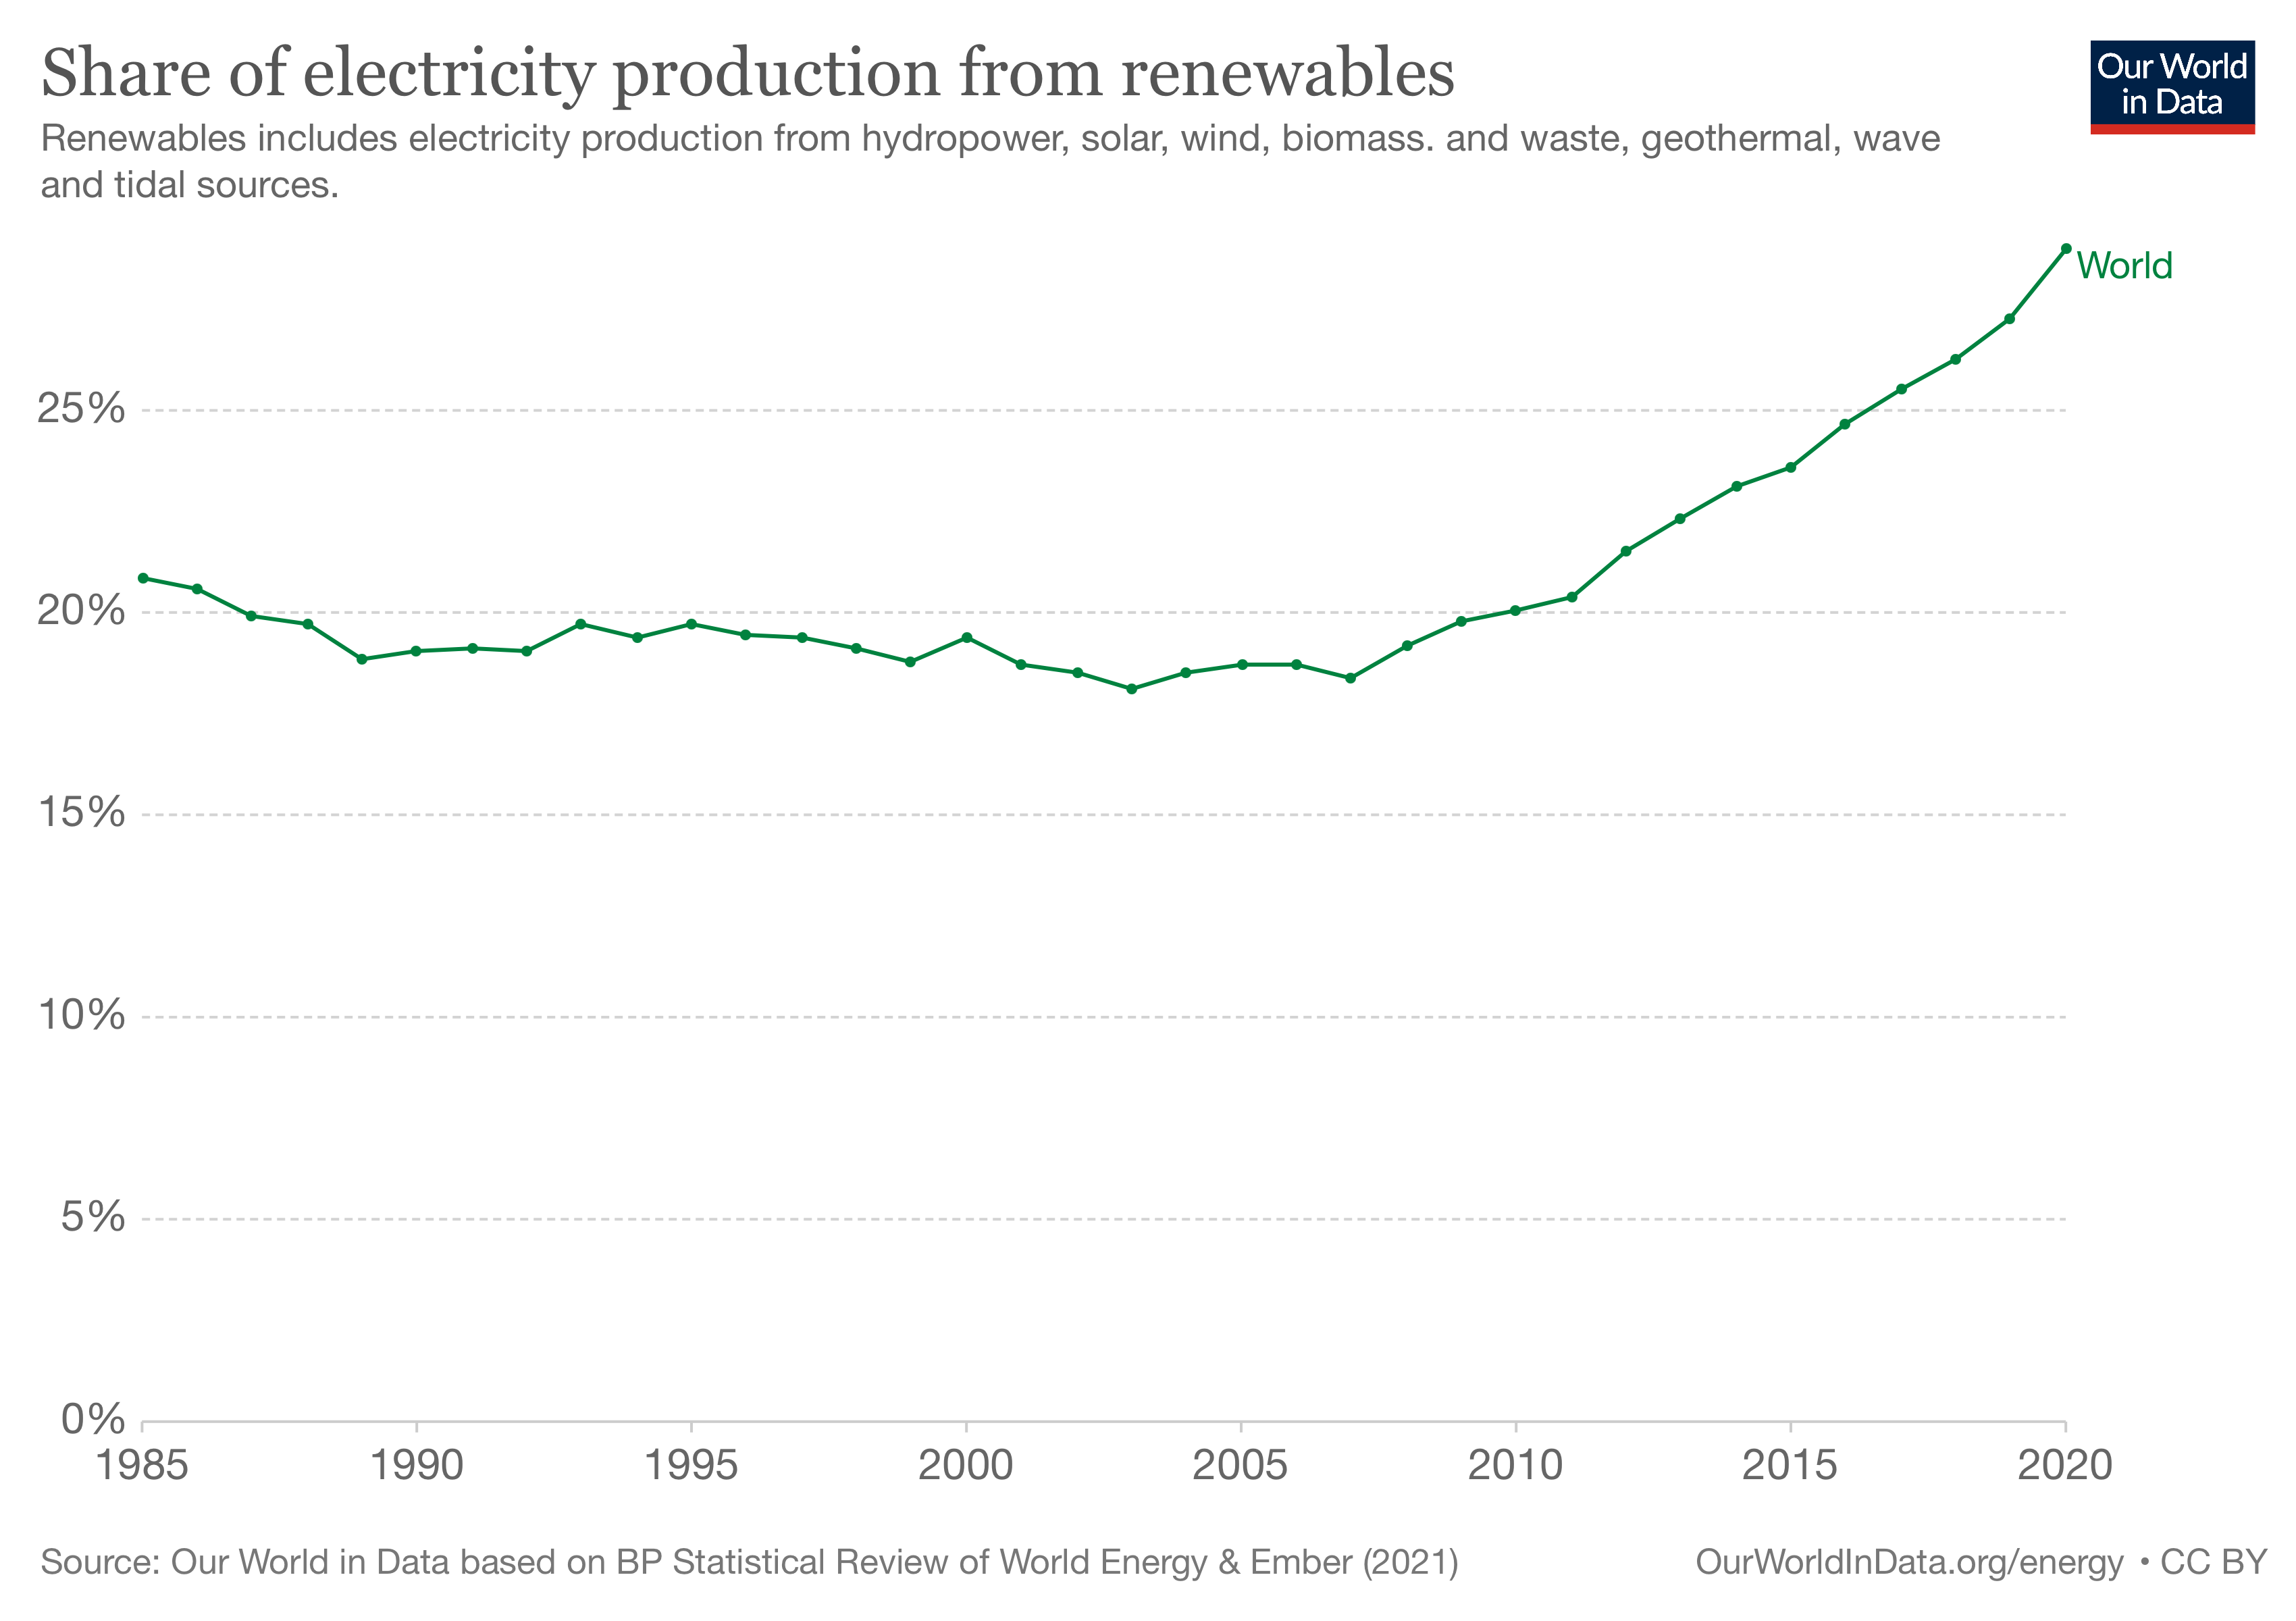
\includegraphics[scale=0.11]{img/intro_renewable.png}
\caption{The share of electricity production from renewables increased from around 18\% to 21\% during 1985 to 2007~\cite{BP2021bp}. The share of electricity production from renewables has been continued growing since 2007. In 2020, the share of electricity production from renewables was around 29\%.}
\label{intro_renewable} % Figure 1.1

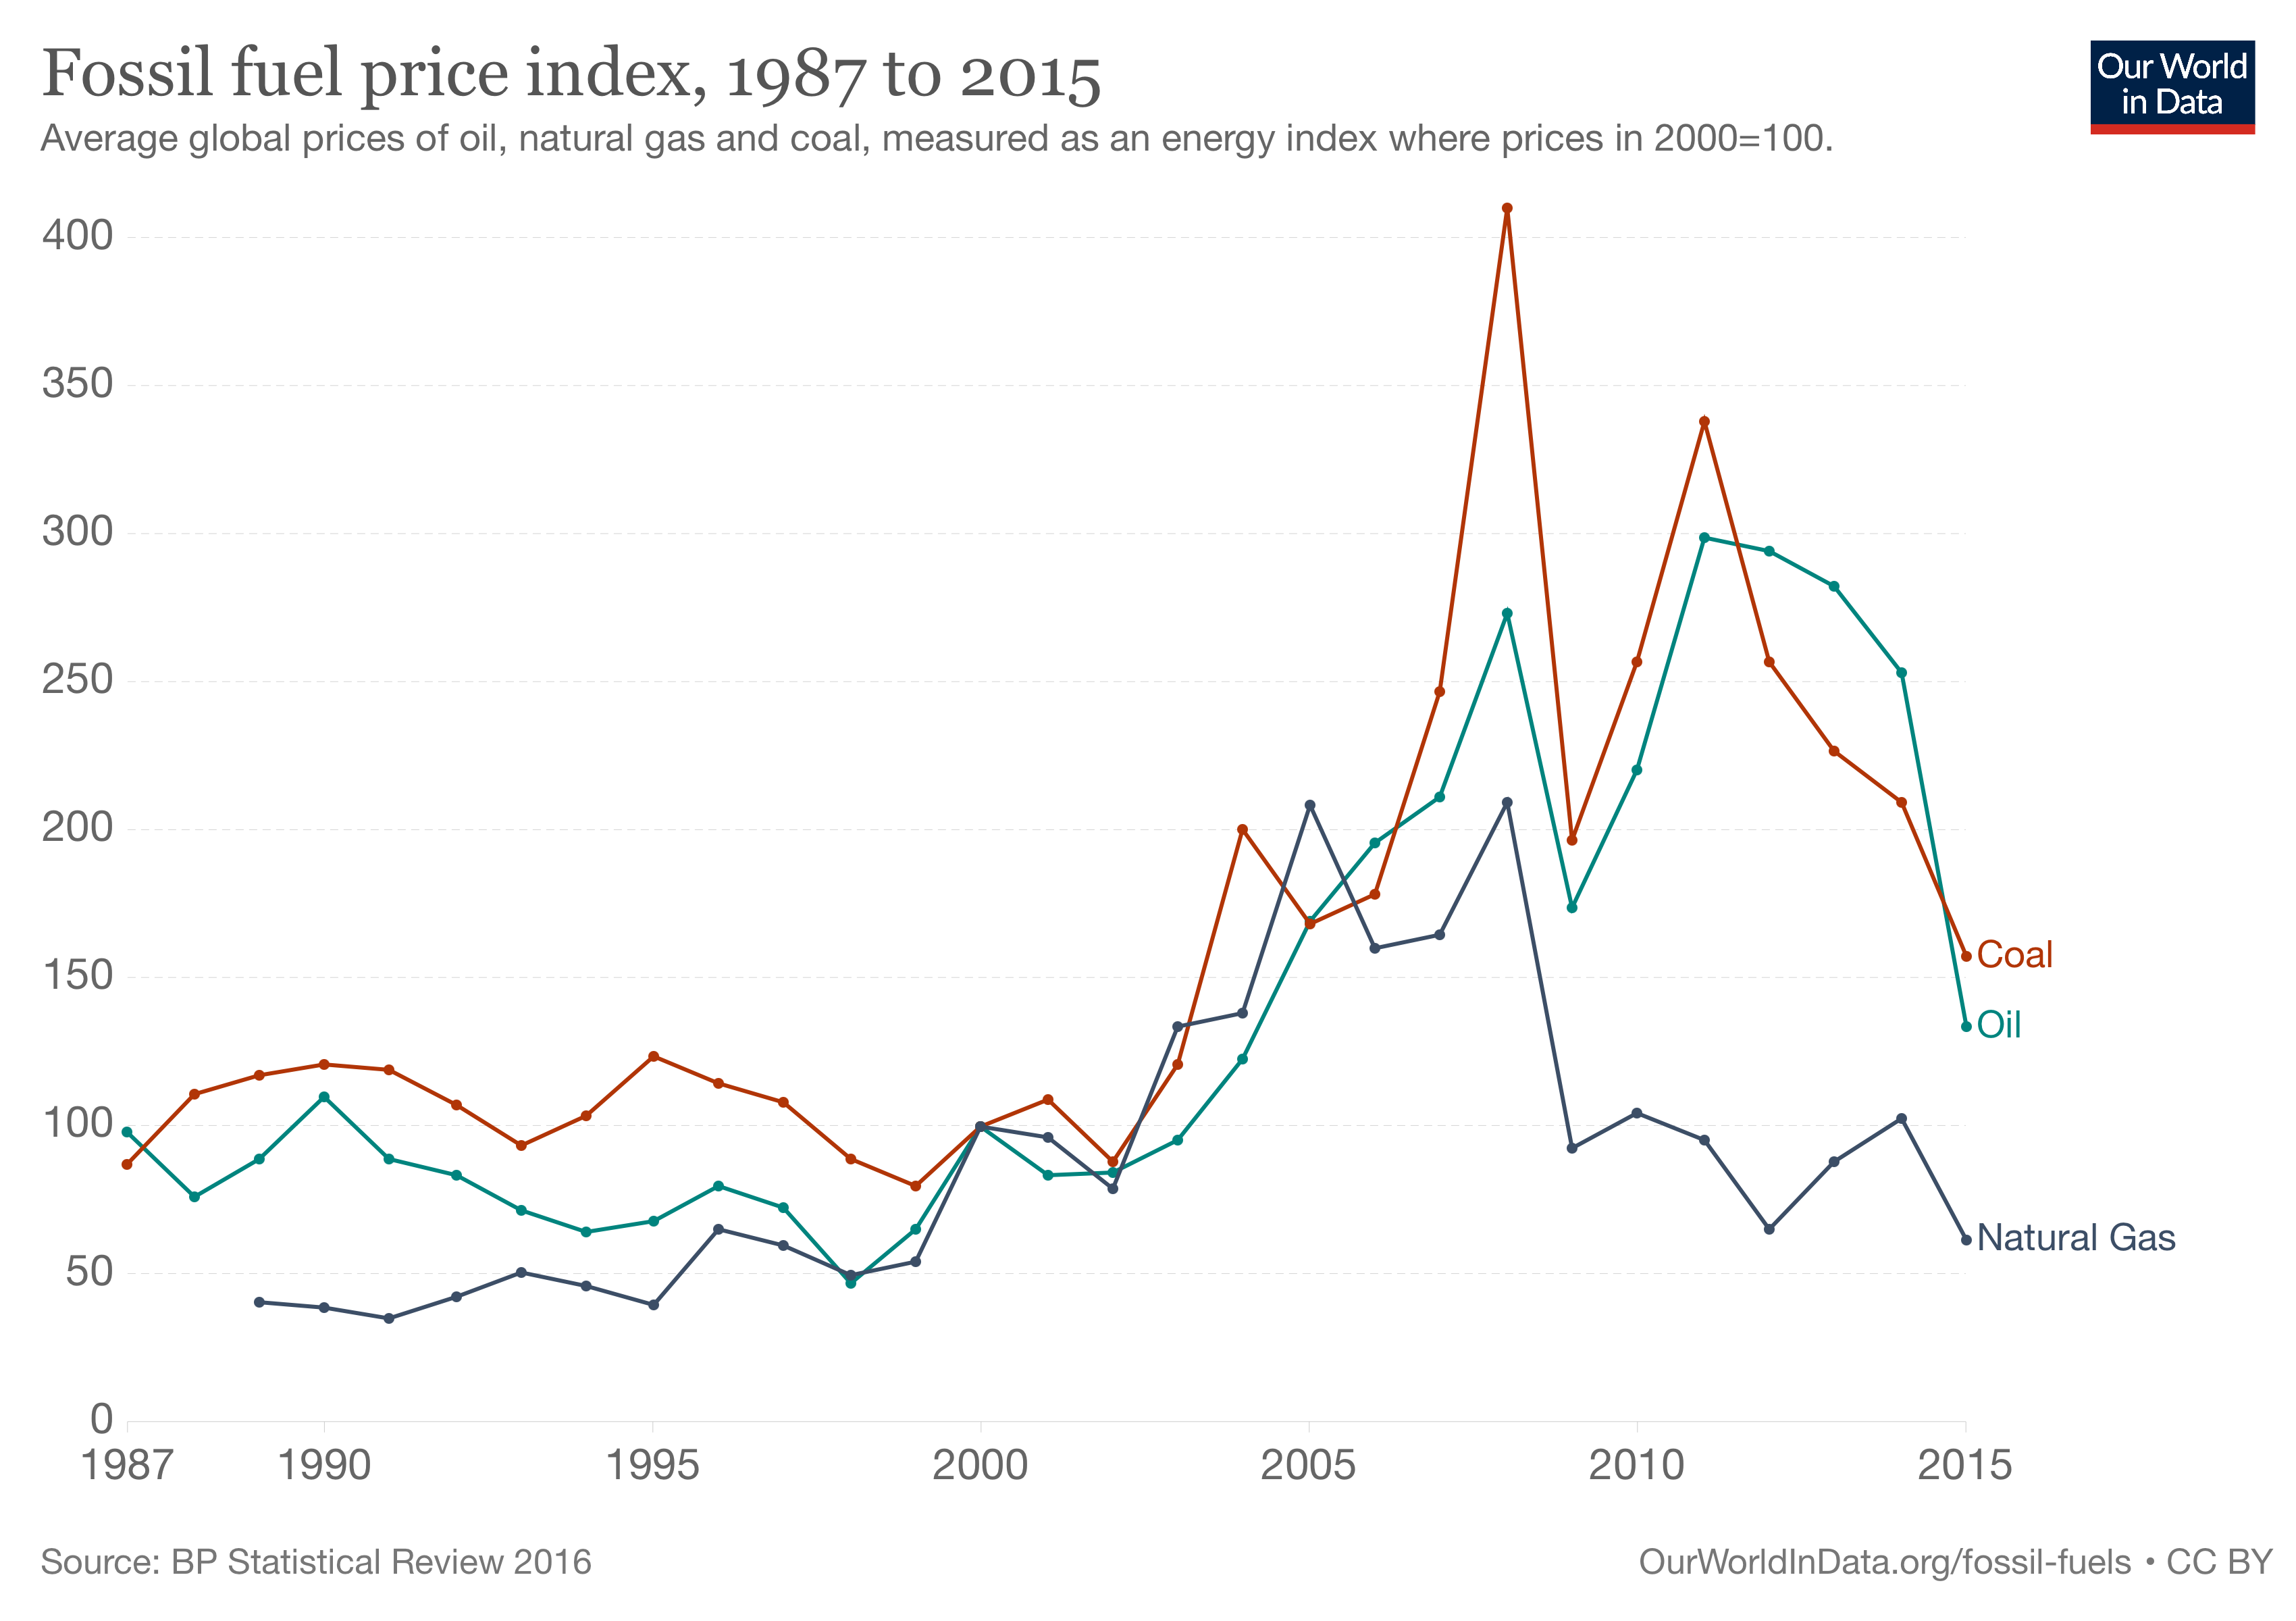
\includegraphics[scale=0.11]{img/intro_fossil-fuel-price-index.png}
\caption{Prices of different fossil fuels rose from 1987 to 2015 overall~\cite{BP2016bp}.}
\label{intro_fossil-fuel-price-index}
\end{figure} % Figure 1.2

Although we might not meet the complete depletion of non-renewable resources in the future 50 years, based on Hotelling’s "Economics of Exhaustible Resources", David Ricardo proposed that as the historical production stock accumulates, higher grade ores get depleted, and the producer resorts to lower grade ores, sustaining greater extraction costs~\cite{devarajan1981hotelling}. It means the extraction costs rise, and the price of the products based on ores will rise as well. Thus, we can assume that the price of most non-renewable resources, like oil, coal and gas, will rise since these have similar properties with ores. In fact, according to BP Statistical Review 2016, from 1987 to 2015 (from 1989 to 2015 for natural gas), the price of oil, coal and natural gas rose by approximately 36\%, 81\%, and 53\% overall (Figure~\ref{intro_fossil-fuel-price-index}). \\

The climate on the earth has changed throughout history. Just in the past 650,000 years, there were seven-cycle glaciers to advance and retreat. As shown in Figure~\ref{intro_co2-concentration-long-term}, however, atmospheric \ce{CO2} had never been above 300 parts per million until the year 1950. According to the paper from Nature, the climate has been changed differently from other periods that happened in the past 70 years~\cite{parmesan2003globally}. It has already had effects on the environment around us. Glaciers are shrinking, and ices are breaking up earlier on the lakes and rivers. Most climate scientists agree that it is human activities that cause global warming~\cite{epic337530}. The atmospheric concentration of \ce{CO2} has been risen for around 36\% since 1914 (see Figure~\ref{intro_co2-concentration-long-term}). As we know, \ce{CO2} is a significant component of the atmosphere. More than a third has increased atmospheric \ce{CO2} concentration since the Industrial Revolution began~\cite{epic337530}. More importantly, as shown in Figure \ref{intro_nasa_co2}, atmospheric \ce{CO2} has exceeded the highest level in the past 400,000 years, and it was 408.52 ppm in 2018. \\

\begin{figure}
\center
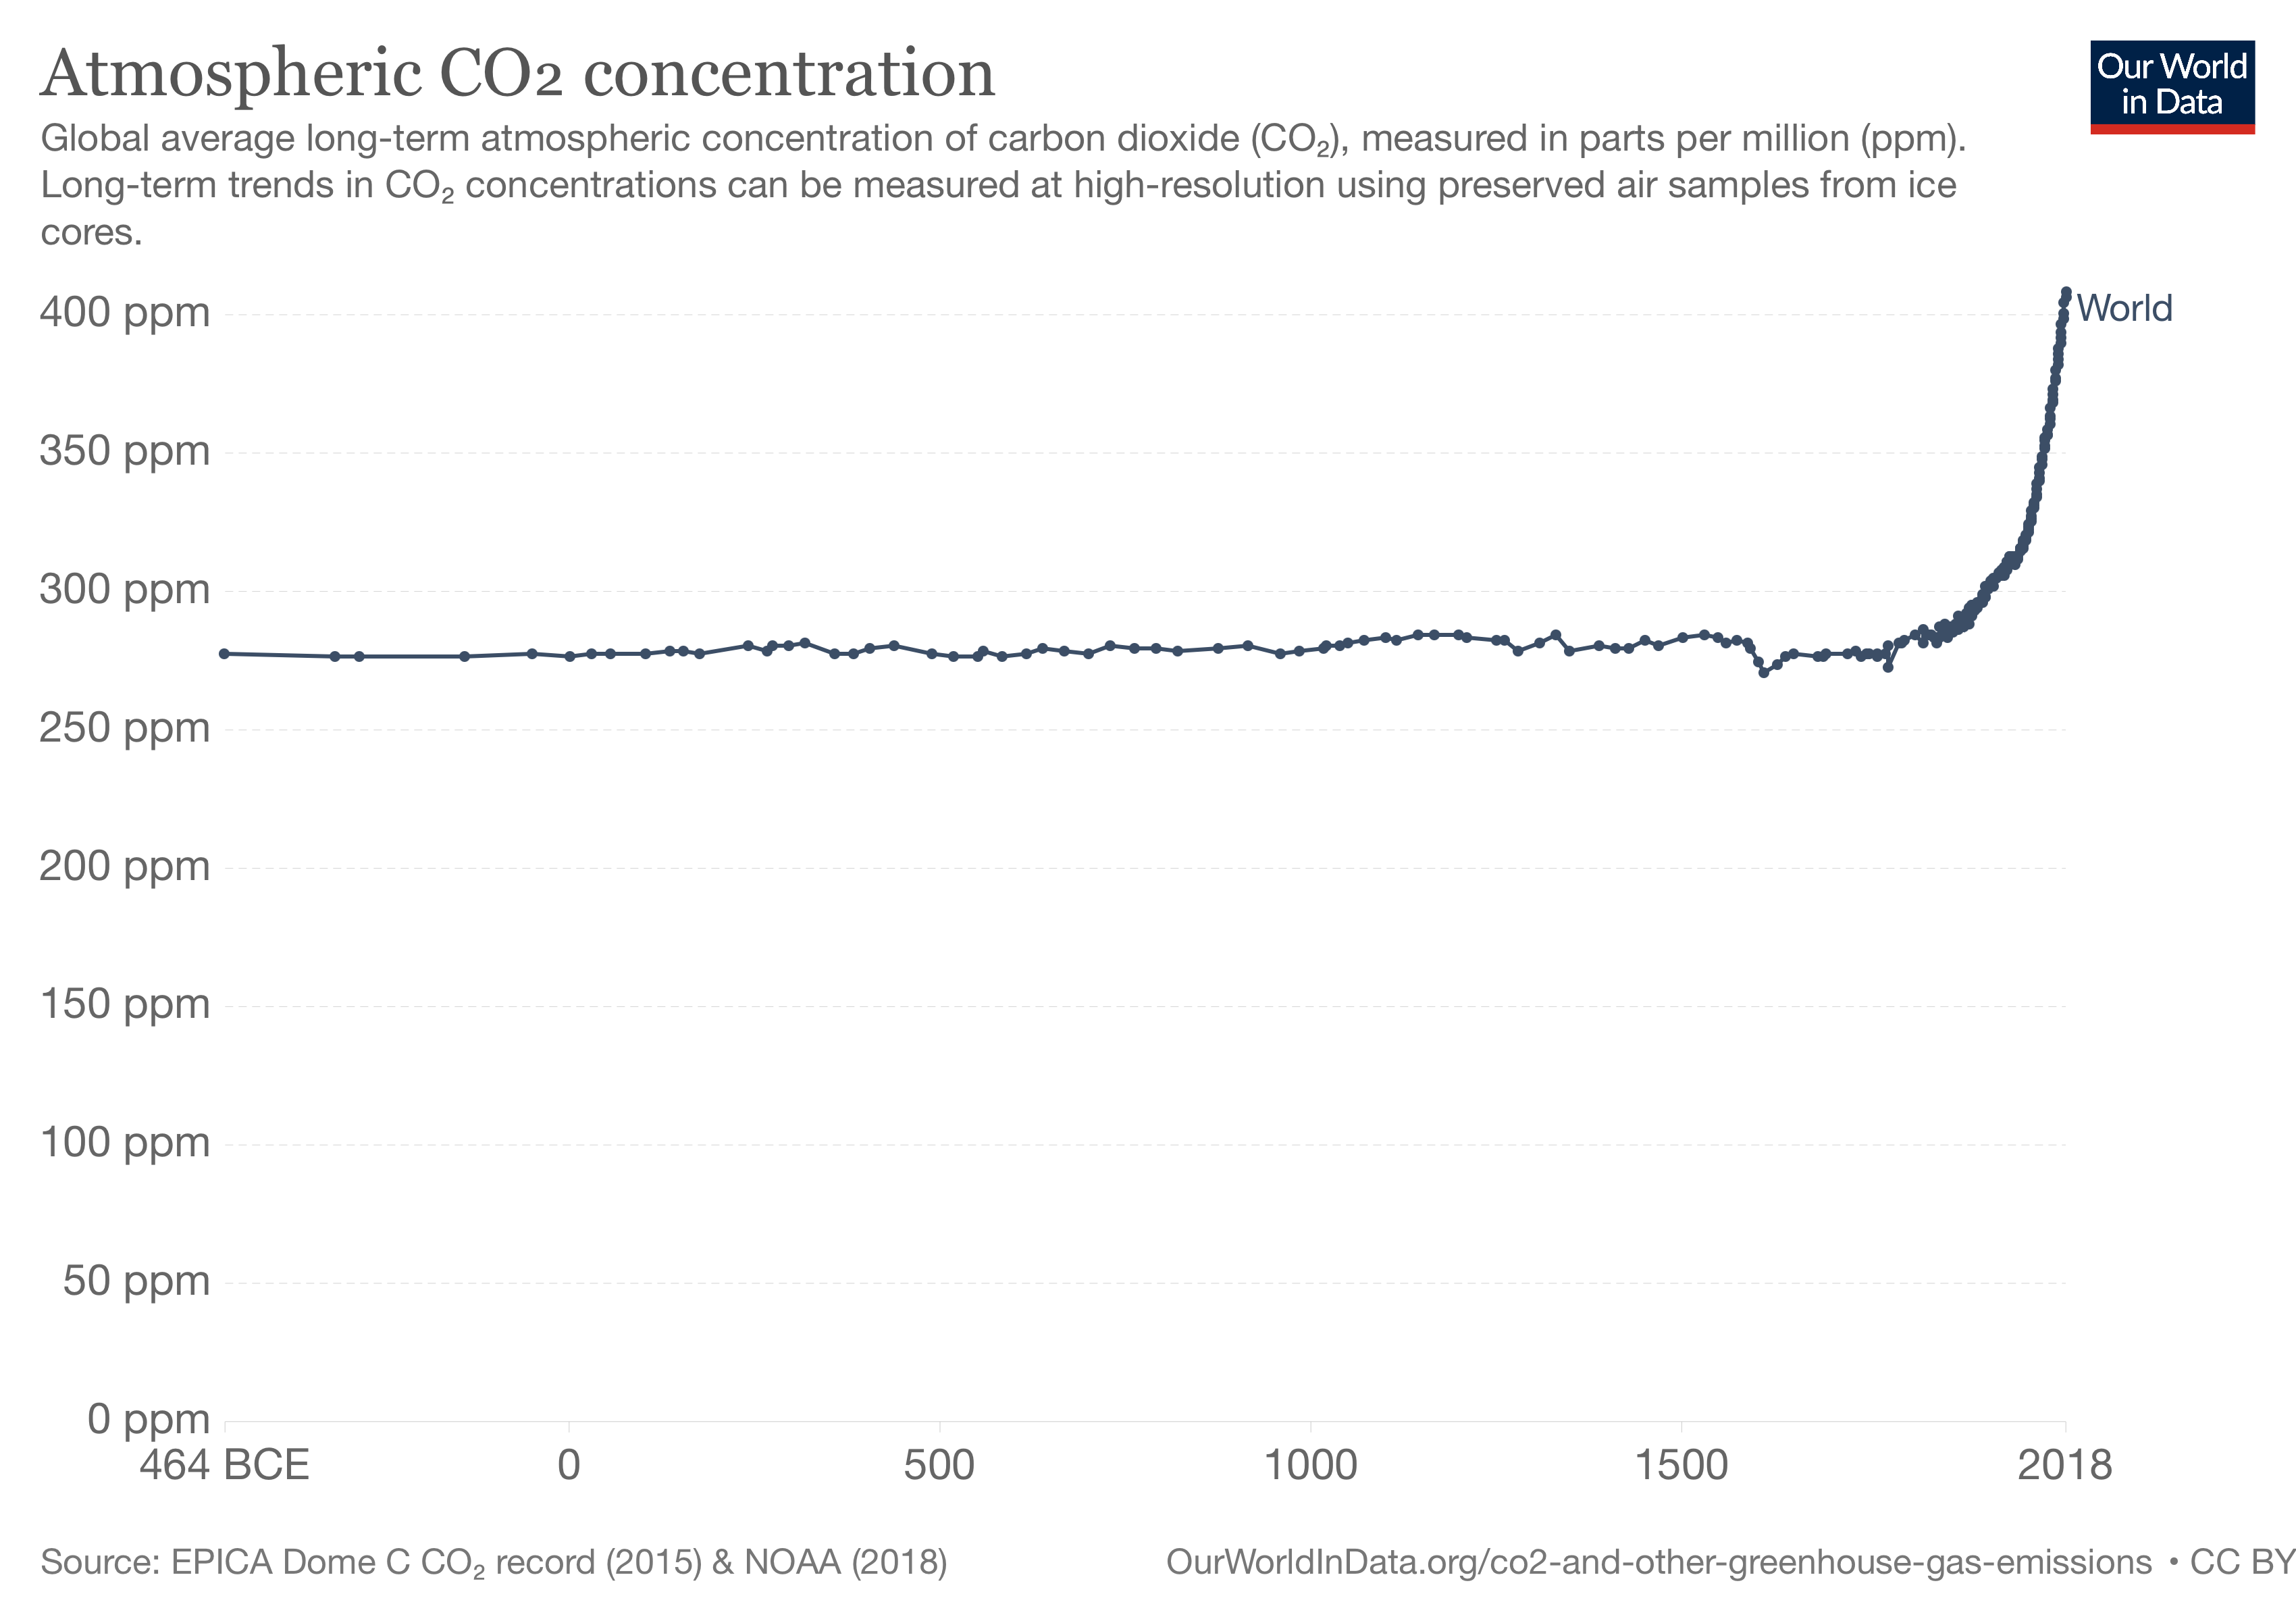
\includegraphics[scale=0.12]{img/intro_co2-concentration-long-term.png}
\caption{Atmospheric concentration of \ce{CO2} since 564 BCE~\cite{bereiter2015revision}. Atmospheric concentration of \ce{CO2} in 1914: 300.17ppm; Atmospheric concentration of \ce{CO2} in 2018: 408.52ppm.}
\label{intro_co2-concentration-long-term}

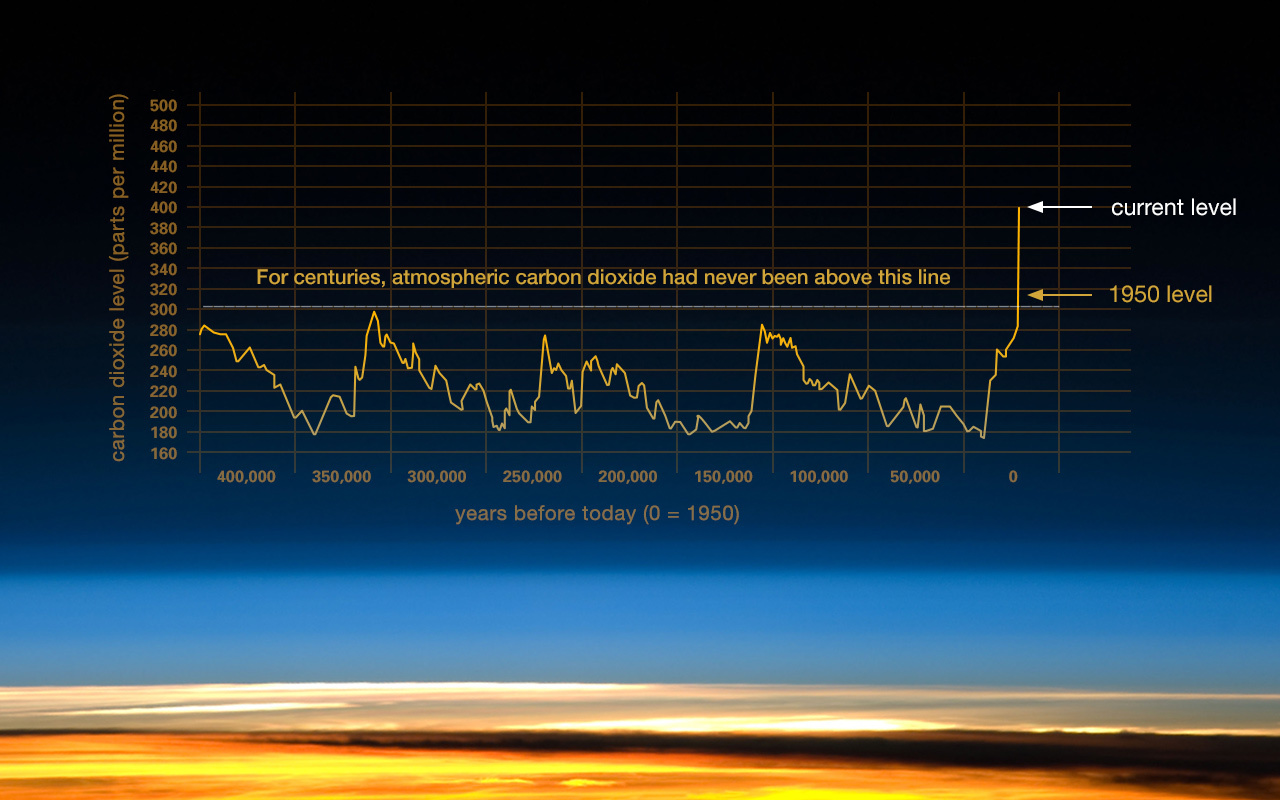
\includegraphics[scale=0.33]{img/intro_nasa_co2.jpeg}
\longcaption{The evidence that atmospheric \ce{CO2} has increased since the Industrial Revolution began}{\label{intro_nasa_co2} The evidence that atmospheric \ce{CO2} has increased since the Industrial Revolution began. Image courtesy: https://climate.nasa.gov/evidence}
\end{figure}


In summary, the rising energy demand and lack of energy supply may cause a short-term energy crisis. The finite resources of fossil energy will drive the price of electricity and consumer goods to rise. The burning of fossil energy will cause excessive emissions of greenhouse gases, leading to global warming. However, a door opens for cheaper but unpredictable renewable energy due to a more expensive fossil fuel. According to Paris Agreements~\cite{unies2015accord}, it is vital to reduce the emissions of fossil energy on a large scale in every sector of human activities. To respond to climate change, supporting the United Nations Sustainable Development Goals and taking urgent action to address climate change and its impact, the International Maritime Organization has formulated a timetable to reduce greenhouse gas emissions from international shipping.~\cite{joung2020imo} It pointed out that between 2030 and 2050, the carbon intensity of the fleet will be reduced by at least 70\%~\cite{joung2020imo}. Before 2050, the total annual greenhouse gas emissions will be reduced by at least 50\%, which requires a reduction of approximately 85\% of carbon dioxide per ship~\cite{joung2020imo}.\\ 

\subsection{Small-Boat Fleet and Emission Inventory}
In 2018, total shipping \ce{CO2} emissions increased to 1056 million tonnes compared to 962 million tonnes in 2012~\cite{IMO2021Fourth}.
In 2016, total \ce{CO2} emissions of the industrial fishing sector were 159 million tonnes, and the small-scale fishing sector emitted 48 million tonnes~\cite{GREER2019103382}. Suppose the increase rate of \ce{CO2} in 2018 was the same as the rate in 2016, and the ratio of the number of small boats and the number of boats can be approximate as the ratio of the number of small fishing boats and the number of fishing boats. Then in 2018, the total \ce{CO2} emissions for the small boat fleet can be calculated as 318.8 million tonnes.\\

Small vessels are classified as those smaller than 24 meters~\cite{uk2021Operational}. Knowing the emissions inventory of the shipping sector can help to understand what measures need to be taken to enable the industry to start the road to full decarbonization. Although it is possible to calculate large vessels from the international registry system and use the satellite data sent from the ship's transponder to account for the numbers of the large vessels~\cite{IMO2021Fourth}, the small vessels depend on the national registration system, and their operation is assumed. In addition, there are many types of small vessels fleets such as machinery (e.g. fishery, people carrier, etc.), hull shape and structure, and the activities of owners and operators. The diverse small boat fleet operational profile is increasing the challenge of accurately accounting for their emission inventories.\\

Emissions from the global fishing industry grew by 28\% between 1990 and 2011, with a minor coinciding increase in production; however, marine fisheries are typically excluded from international assessments of \ce{CO2} or are generalized based on a limited number of case studies~\cite{parker2018fuel}. Developed economies such as the UK have a national registry~\cite{uk2021registration} that allows to have a sense of the level of small boat activity and hence infer the \ce{CO2} emissions.\\

However, in developing countries, it tends to be a mixed bag on the level of precision and availability. For instance, in Mexico, only fishing vessels are counted into registry~\cite{Mexico2021RegisteredVessels}. Still, it is difficult to know where they are located. Besides, the rest of the small-boat fleets are not considered. In all, Mexico does not have a regional \ce{CO2} inventory considering the small-boat fleet. Therefore, quantifying the number of small-boat fleets will allow a better precision of where the emissions are being emitted and will be the focus of understanding the emission inventory of the shipping sector.\\


Observing the shipping activity in the Gulf of California is essential due to its unique geographical location, conformation, and biophysical environment ~\cite{LLUCHCOTA20071, munguia2018ecological, MARINONE2012133}. In the Gulf of California, there is the largest fish producing state (Sonora) in Mexico~\cite{MELTZER2006222} and the most prominent sports fishing destination (Los Cabos, Baja) in Mexico~\cite{hernandez2012economic}. Besides, the Gulf of California has a faster shipping route to mainland Mexico than from Yucatán Peninsula.\\

\subsection{Bringing Image Recognition in Satellite Images Detection}

\section{Research Questions}


\section{Thesis Outline}


\section{Contributions}


% Literature Review
\chapter{Literature Review}
\label{chapter:Review}
%!TEX root = thesis.tex

\section{Small Boat Fleet and Shipping Decarbonisation}
Current literature related to estimating small-scale vessels without machine learning methods includes using statistical factors or measures.~\newcite{johnson2017spatial} used Kernel Density Estimation (KDE) to distribute data on the population, the number of ships, and the average annual total catch for the entire population, and finally showed that their forecasts could accurately predict the landing of fisheries in the bay. In their paper, they explained the source of their data~\cite{Lopez-Sagastegui2017Comparing}. Lopez-Sagastegui et al. worked with fishermen to generate and record information about fish catches, fishing effort, profits, species breeding seasons, and spatial patterns of fishing activities. However, one of the points to make against this work is that it only focuses on fishing vessels. While these are the majority, it still misses the other ship types. Notably, the authors provided information (Figure~\ref{review_density_of_gulf}) of the density of human population and boats in the Gulf of California that can save much time in creating data sets of the Gulf of California for training machines learning models.\\

\begin{figure}[t]
\center
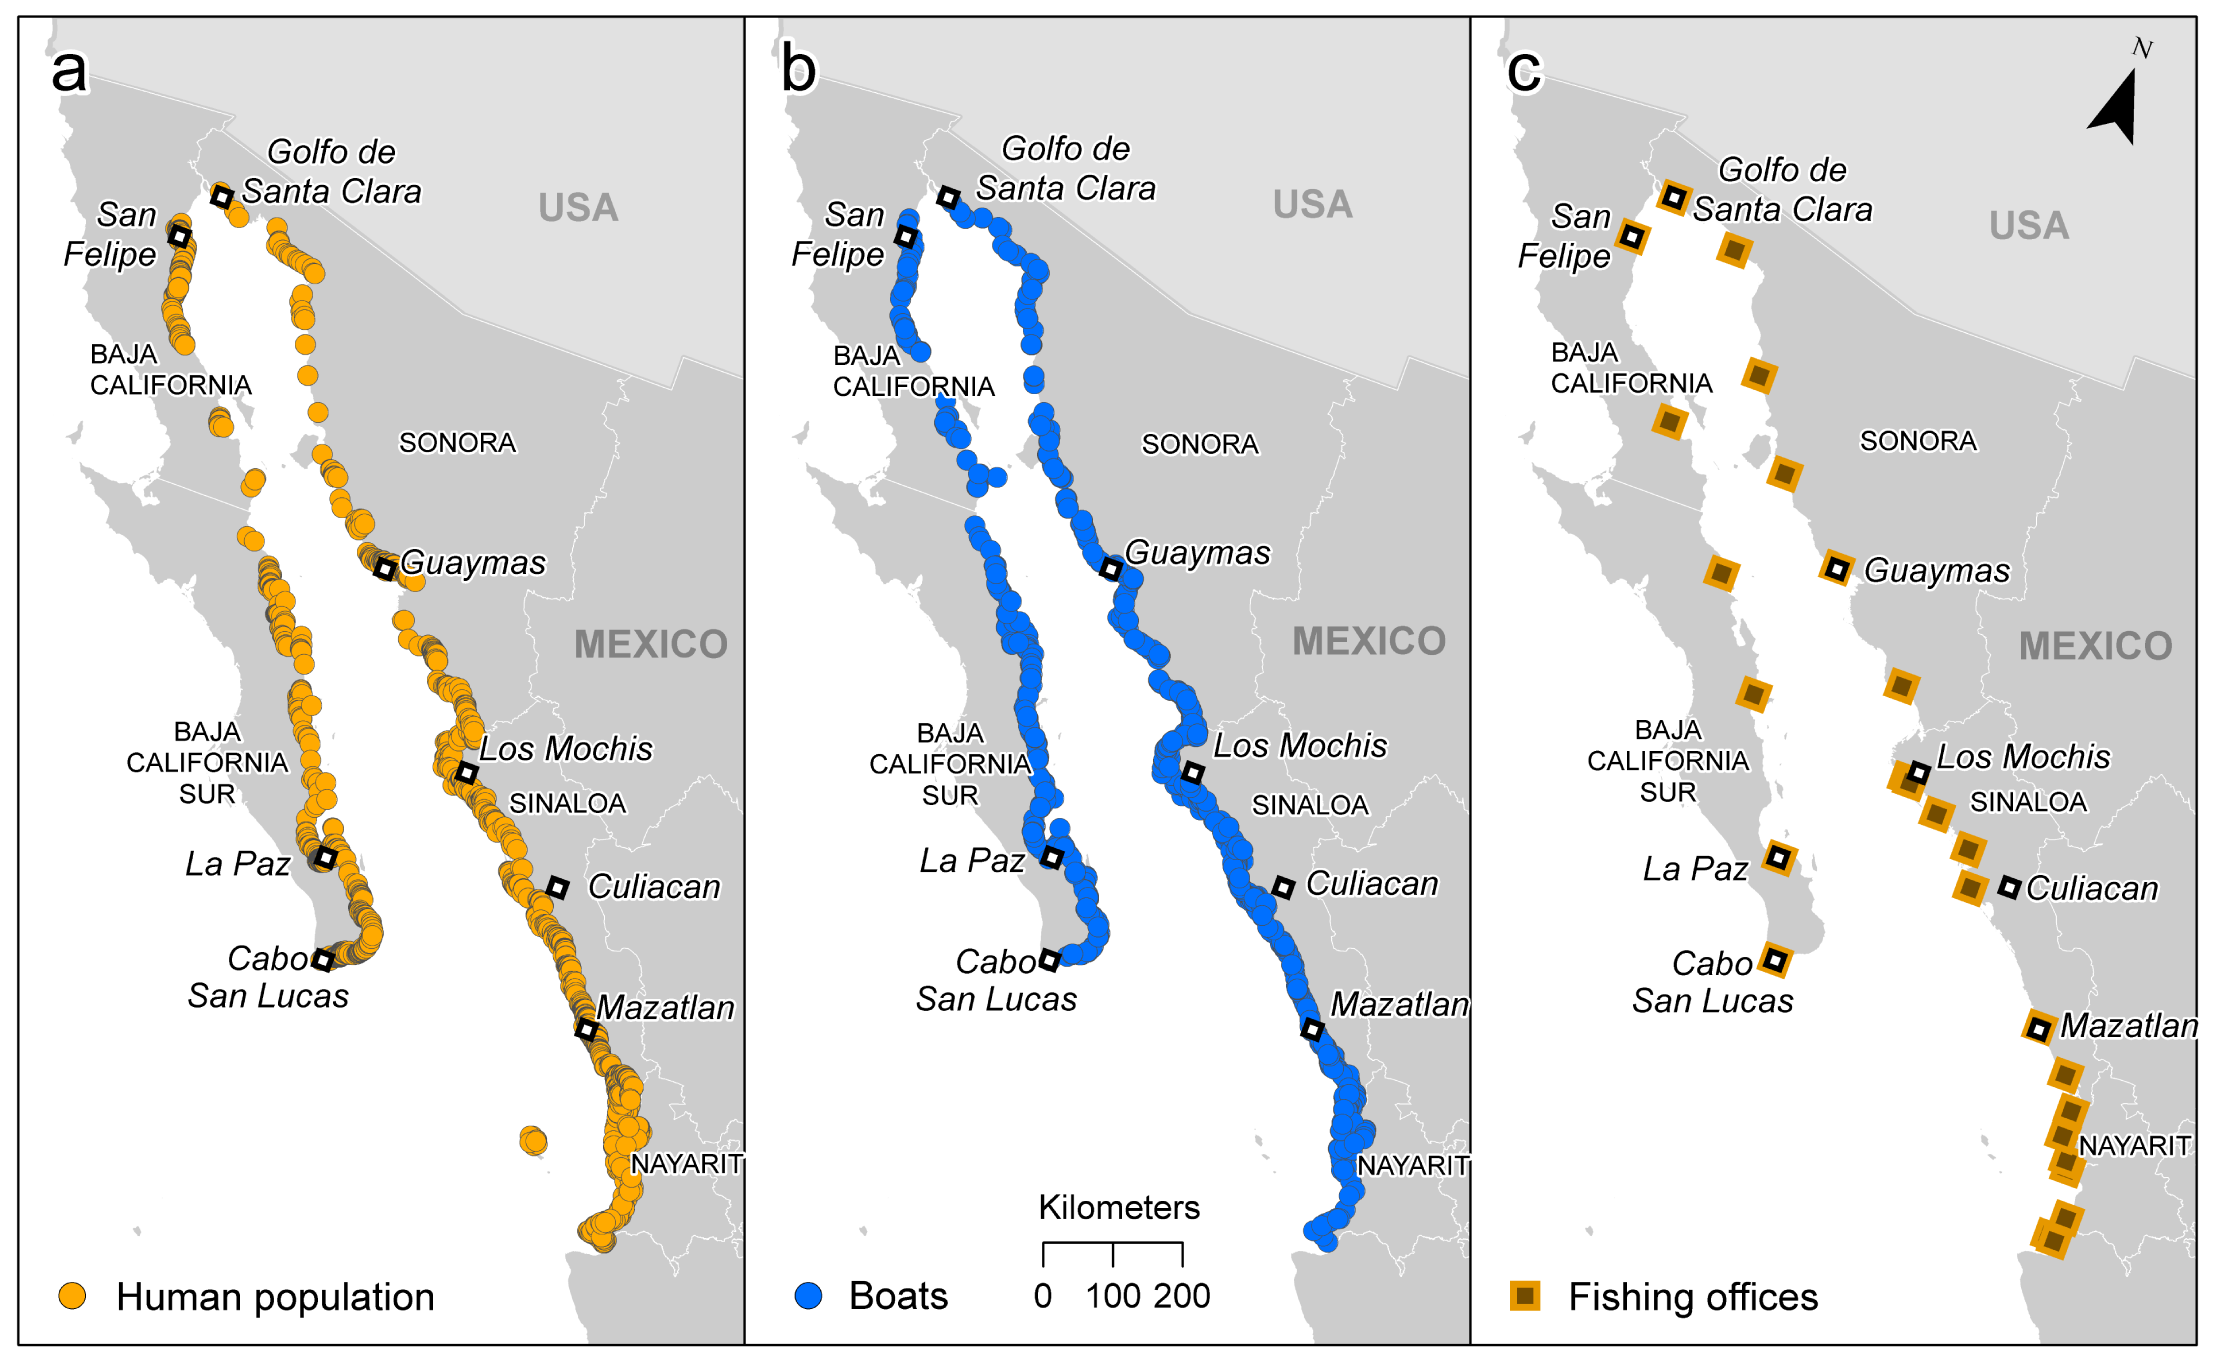
\includegraphics[scale=0.83]{img/review_density_of_gulf.png}
\longcaption{Map of the density of human population, boats, and fishing offices in the Gulf of California.}{\label{review_density_of_gulf} Map of the density of human population, boats, and fishing offices in the Gulf of California. Image courtesy: https://doi.org/10.1371/journal.pone.0174064.g002}
\end{figure}

~\newcite{Johansson2018ModelingOL} proposed a new model (FMI-BEAM) to describe the emissions of the leisure boat fleet in the Baltic Sea region with over 3000 dock locations, national small boat registry, AIS data and vessel survey results. However, the method cannot cover countries with no national registry for small boats. Besides, small boats are not just leisure boats.~\newcite{Ug2020EstimationOW} estimated global ship emissions with the help of data from the Automatic Identification System (AIS). They set up movement information relating to ship size and speed and meteorological and marine environmental conditions. Over 3,000,000,000 daily AIS data records from hundreds of owners and thousands of partner AIS base stations and detailed ship data. However, this method is highly dependent on AIS data which is impossible for unregistered small boats.~\newcite{Traut2013MonitoringSE, Johansson2016ACM, Mabunda2014EstimatingCD, Hensel2020GreenSU, Han2016RealtimeIA} have proposed the use of AIS to monitor the carbon emissions of the fleet as well.\\

~\newcite{Zhang2019TheSO} included unidentified vessels in the AIS-based vessel emission inventory. They developed an AIS-instrumented emissions inventory, including both identified and unidentified vessels. In particular, missing vessel parameters for unidentified vessels were estimated from a classification regression of vessels with similar vessel types and sizes in the AIS database. However, the authors do not discuss whether the regression model applies to vessels in most coastal areas of the planet. In addition, the authors do not discuss whether the vessel data in the AIS database is regionally diverse. Finally, if there is a diversity of vessels in the AIS database, the authors did not discuss whether this diversity would produce more significant errors in the predictions for small vessels in a single region (e.g. the Gulf of California, Mexico).


\section{Convolutional Neural Networks in Image Recognition}
\label{sec2.2}
Literature tends to be inaccurate for emission inventories for the small boat fleet. The above literature review has demonstrated that there is still a lot of work to do in order to understand how the small boat fleet is being operated, what fuels they are using and the level of activity for this shipping sector. This master thesis project intends to use image recognition algorithms for the identification of small boats in any sea area, significantly reducing the time taken to calculate small vessel emission inventories. Besides, it will be in the national interest for the small fleet to account for and control these emissions within the powers of the state, incentivising the energy-efficient technologies and fuel change. Further, if countries are to meet their ambitious net-zero carbon emissions targets, they cannot afford to ignore the small boat fleet emission inventories that can help governments account for carbon emissions from small boats more quickly.\\

Object detection is an active topic in image recognition and computer vision. In the past few years, this topic has made significant progress. With the rise of self-driving cars and face detection, there is an increasing demand for fast and accurate objects detection. In 2012, AlexNet won the ImageNet Large-Scale Visual Recognition Challenge (ILSVRC), making convolutional neural networks the dominant mode of image recognition~\cite{krizhevsky2012imagenet}. Then,~\newcite{girshick2014rich} introduced R-CNN, which is the first CNN-based object detection method, but with higher performance.\\

Unlike other deep learning problems, the unknown number, size and categories of instances in each image in the object detection problem lead to unexplored dimensions of the model output. Therefore, it is not easy to adapt the classic deep learning classification model that expects a fixed output size to the object detection problem. Region-Based Convolutional Neural Networks (R-CNN) may be the way to meet this challenge.\\

Since its inception, Region-Based Convolutional Neural Networks (R-CNN) has gone through many iterations: R-CNN, Fast R-CNN, Faster R-CNN and Mask R-CNN~\cite{girshick2014rich, girshick2015fast, ren2015faster, he2017mask}. To avoid computationally expensive, pixel-level classification and object search, the original R-CNN method applied a non-deep learning algorithm called Selective Search to obtain approximately 2000 region suggestions~\cite{uijlings2013selective, girshick2014rich}. Then, with the help of a modified version of the AlexNet model, features are extracted from the proposed region. The objects in the image have different scales and sizes, so their corresponding image crops need to be warped to fit the following CNN input size. Then, the support vector machine (SVM) classifier uses the extracted features for classification, and the linear regression predicts the offset of the bounding box, thereby tightening the bounding box around the object~\cite{girshick2014rich}.\\

R-CNN is an intuitive architecture that has achieved high accuracy in object detection. However, since the reasoning time for each image is about 30 seconds, this model is very inefficient for applications that require real-time prediction~\cite{huang2017speed}. Fast R-CNN performs feature extraction on the image before generating the region suggestion. The region suggestion is generated based on the final feature map instead of the original image itself, significantly improving the training and inference speed. Therefore, only one CNN forward channel is calculated on the entire image, instead of about 2000 channels as it is now. Although Fast R-CNN does improve efficiency, selective search to generate region recommendations is the most computationally intensive part of the architecture, which forms a bottleneck in network inference and training time. Faster R-CNN alleviates this problem by replacing the selective search algorithm with a neural network called a region proposal network (RPN). The network simultaneously predicts the boundaries of objects and the classification between the two types of objects at each location and the background~\cite{ren2015faster}. The rest of the architecture is similar to that proposed by Fast R-CNN.
A recently proposed architecture, Mask R-CNN~\cite{he2017mask}, can perform object detection in addition to instance segmentation by adding a fully convolutional network (FCN) branch to the Faster R-CNN architecture. Instance segmentation can be defined as demarcating and classifying object instances belonging to different categories in the image.\\

However, even traditional CNNs can be very useful for large-scale image recognition.~\newcite{Simonyan2015VeryDC} in the University of Oxford, and Google DeepMind researched the effect of convolutional network depth on its accuracy in the large-scale image recognition setting. Their research found out that even they used very small (3x3) convolution filters, a significant improvement can be achieved by pushing the depth to 16 to 19 weight layers.\\


\section{Noise Removal for Image in the Shipping Sectors or Similar Applications}
Satellite images often have targets that should not be there, such as shadows cast by water on the sea surface due to sunlight or clouds in the atmosphere. These noises can make the training data inaccurate and often cause problems for the correctness of the model.~\newcite{He2009SingleIH} proposed a simple but effective image prior-dark channel before removing haze from a single input image. The dark channel prior is a kind of statistics of outdoor haze-free images. It is based on critical observation-most local patches in outdoor haze-free images contain some pixels whose intensity is very low in at least one colour channel. Using this prior to the haze imaging model, the thickness of the haze can be estimated, and a high-quality haze-free image can be recovered. Moreover, a high-quality depth map can also be obtained as a byproduct of haze removal.\\

% Methodology
\chapter{Methodology}
\label{chapter:Methodology}
\label{chap:3}
\section{Artificial Intelligence Framework}
\label{sec:3.1}
\subsection{The Algorithm: Deep Learning Architecture (CNN/ConvNet)}

Neural networks originate from the human perception of the brain. In 1943, American neuroscientists McCulloch and Pitts proposed a theory that every neuron is a multiple-input single-output structure~\cite{mcculloch1943logical}. And there are only two possibilities for this output signal, it's either zero or one, which is very similar to a computer.\\

In image recognition, if we have a 7x7 image, this 7x7 image has 49 elements. If we write down an `X' in this grid, as shown in Figure~\ref{fig:x_7x7_image}, in the computer's view, it is actually a series of numbers. If each cell is either black or white, for example, black is 1 and white is 0, so what it represents could be a 7x7 matrix, as shown in Figure~\ref{fig:x_7x7_matrix}.\\


\begin{figure}[!tbp]
  \centering
  \begin{minipage}[b]{0.4\textwidth}
    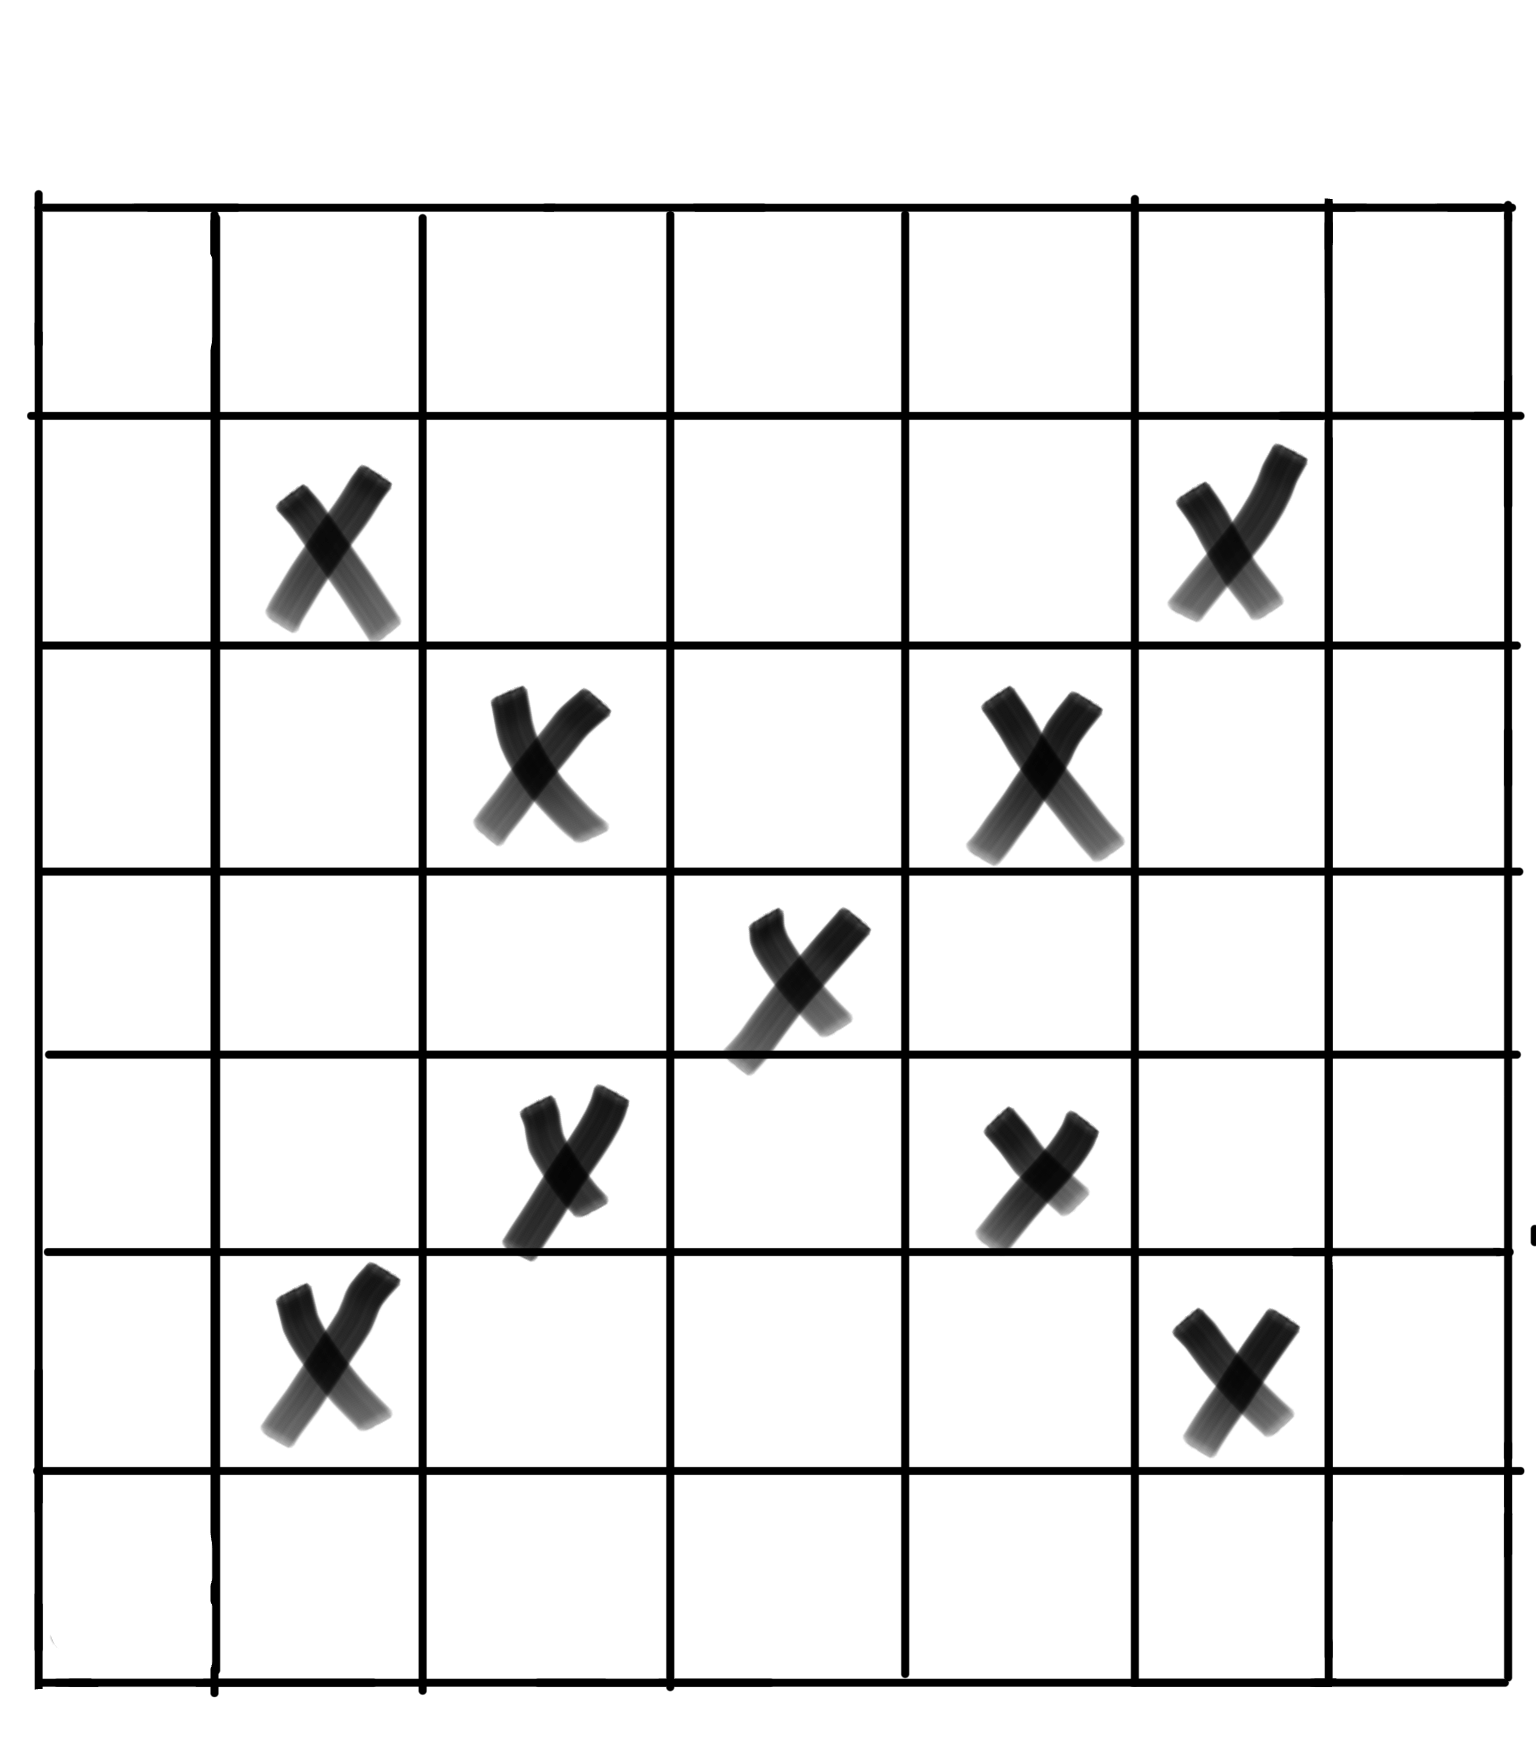
\includegraphics[width=\textwidth]{img/X.png}
    \caption{Letter X in a 7x7 image.}
    \label{fig:x_7x7_image}
  \end{minipage}
  \hfill
  \begin{minipage}[b]{0.4\textwidth}
    \centering
    $\begin{bmatrix}
    0 & 0 & 0 & 0 & 0 & 0 & 0\\
    0 & 1 & 0 & 0 & 0 & 1 & 0\\
    0 & 0 & 1 & 0 & 1 & 0 & 0\\
    0 & 0 & 0 & 1 & 0 & 0 & 0\\
    0 & 0 & 1 & 0 & 1 & 0 & 0\\
    0 & 1 & 0 & 0 & 0 & 1 & 0\\
    0 & 0 & 0 & 0 & 0 & 0 & 0
    \end{bmatrix}$
    \caption{Letter X in a 7x7 matrix.}
    \label{fig:x_7x7_matrix}
  \end{minipage}
\end{figure}


\begin{figure}[!tbp]
  \centering
  \begin{minipage}[b]{0.4\textwidth}
    \centering
    $\begin{bmatrix}
    1 & 0 & 0\\
    0 & 1 & 0\\
    0 & 0 & 1
    \end{bmatrix}$
    \caption{A 3x3 convolution kernel.}
    \label{fig:3x3_convolution_kernel}
  \end{minipage}
  \hfill
  \begin{minipage}[b]{0.4\textwidth}
    \centering
    $\begin{bmatrix}
    2 & 0 & 1 & 0 & 1\\
    0 & 3 & 0 & 1 & 0\\
    1 & 0 & 3 & 0 & 1\\
    0 & 1 & 0 & 3 & 0\\
    1 & 0 & 1 & 0 & 2\\
    \end{bmatrix}$
    \caption{A 5x5 feature map.}
    \label{fig:5x5_feature_map}
  \end{minipage}
\end{figure}



After feeding the program as much as data, the program will be trained to find parameters to determine if it is an `X' or not. If it is a grey-scale picture, each number is not 0 and 1, but a grey-scale value from 0 to 255. If it's a colour image, then it's RGB colours. Essentially, no matter what the image is, the image can end up replacing itself with a bunch of numbers, and that a bunch of numbers can be an input of the training neural network. The goal of training is to find the parameters that make the loss function smallest.\\

But if we use the method described above to train real-world images, it is time-consuming and computationally expensive. Besides, once the image is a little bit deflated and rotated, or changed, then the algorithm will not recognize it. But our eyes are very efficient: if I see a car and a motorcycle once, I can immediately tell the difference between them, and the next time I see the motorcycle, even if the motorcycle has changed direction, position, or is broken, we can still recognize it as a motorcycle and not a car.\\


In 1981, the Nobel Prize in Physiology or Medicine was awarded to two neuroscientists, David Hubel and Wiesel. These two scientists experimented with cats, inserting electrodes into their brains and then showing them a variety of different images to study the results of their brain responses~\cite{hubel1962receptive}. They found that there are two types of cortical fields in the brain related to vision. The first one is called `simple cortical fields', which is characterized by sensitivity to certain lines. After the appearance of lines in a certain direction, these fields will be more sensitive and can see it. There are `complex cortical fields' as well. These complex fields are not only able to respond to lines, but it is also able to respond to the movement of the objects.\\


Later, inspired by them, a Japanese scientist named Kunihiko Fukushima proposed a model called the Neocognitron Model, which explains how a person can see whether the object is a cat or a dog~\cite{fukushima1982neocognitron}. He proposed that there are many layers in the human brain. The visual signals are processed layer by layer. After light enters the eye from the outside, it enters the first layer, then the second layer, then the third layer, and so on. Each layer processes the signal differently. In the beginning, when the light enters the retina, the human eye actually sees a large number of pixels. In the first layer, these pixels abstract some features, such as edges. Then the next layer combines these features to form the outline of the object and more details of the object. Finally, the contours and details are combined into a whole to make a final judgment.\\


Based on this principle, Yann LeCun invented a practical method for image recognition, called convolutional neural network~\cite{lecun1995convolutional}. The role of convolution is to use a mathematical method to extract these features from the image. The way to extract the features is to use a convolution kernel to do the convolution operation. The convolution kernel is also a matrix and is usually a 3x3 or 5x5 matrix. For instance, if we have a convolution kernel which is a 3x3 kernel, and the numbers in it are shown in Figure~\ref{fig:3x3_convolution_kernel}, then a convolution operation will be done with this kernel and the matrix shown in Figure~\ref{fig:x_7x7_matrix}. The operation result is shown in Figure~\ref{fig:5x5_feature_map}. This result is also known as a feature map.\\


In fact, the feature map reinforces the features of the convolution kernel. If you look carefully, you will see that this convolution kernel (Figure~\ref{fig:3x3_convolution_kernel}) only has three oblique blocks of pixels being ones. So if the original matrix (Figure~\ref{fig:x_7x7_matrix}) also has oblique pixel blocks of ones, the number would be extensive when they do the convolution operation. That means we have extracted this feature. The smaller the value of the pixel block in the other positions, the less it satisfies the feature. In a word, with different convolution kernels, we can get different feature maps.\\

The next step after convolution is pooling. This feature map (Figure~\ref{fig:5x5_feature_map}) has a relative large number of elements. For instance, the top left corner has a feature of a line to the bottom right. But the presence of `2' and `3' at the top left of the matrix means that the two zeros around them don't really mean much. So we can simplify it by zooming in on the part of this feature map that has features and ignore the part that doesn't have features. We can use a maximum pooling method. That is, we can extract the largest number from these four numbers (2x2 matrix). Eventually, it can be pooled into a relatively small feature map (Figure~\ref{fig:3x3_feature_map_after_pooling}).\\

\begin{figure}[b]
  \centering
  \begin{minipage}[b]{0.4\textwidth}
    \centering
    $\begin{bmatrix}
    3 & 1 & 1\\
    1 & 3 & 1\\
    1 & 1 & 2
    \end{bmatrix}$
    \caption{A 3x3 feature map after pooling.}
    \label{fig:3x3_feature_map_after_pooling}
  \end{minipage}
  \hfill
  \begin{minipage}[b]{0.4\textwidth}
    \centering
    $\begin{bmatrix}
    0.95 & 0.73 & 0.73\\
    0.73 & 0.95 & 0.73\\
    0.73 & 0.73 & 0.88
    \end{bmatrix}$
    \caption{A 3x3 feature map after activating with sigmoid function.}
    \label{fig:3x3_feature_map_after_activating}
  \end{minipage}
\end{figure}

The step after pooling is activation. The essence of the activation function is to introduce nonlinear factors to solve problems that a linear model cannot solve. Suppose the activation function is a sigmoid function, i.e.,

\begin{equation}
    S(x) =  \frac{\mathrm{1} }{\mathrm{1} + e^{-x} }.
\end{equation}

After activating the sigmoid function, each element in the feature map would be between 0 to 1, as shown in Figure~\ref{fig:3x3_feature_map_after_activating}.\\

It is worth noting that the initial convolution kernel may be artificially set. But later on in the process of machine learning, it will go backwards to adjust and find the most suitable convolution kernel based on its own data, just like the above-mentioned method of using training to adjust the parameters is no different. Since a picture will generally have many features, there will be many corresponding convolution kernels. After many times of convolutions and poolings, features can be found, such as the slanted lines of image, the contours, and the colour features. We take this enough information and then feed it into this fully connected network for training, and finally, we can determine what this image really is.\\

In Sec~\ref{sec2.2}, recent literature and development of Convolutional Neural Networks were discussed. However, a number of convolutional neural network-based object detection frameworks have recently emerged that can run faster, have a higher detection accuracy, have cleaner results and are easier to develop. Contrastingly, compared to the Faster RCNN model, the YOLO model can better detect smaller objects, for example by easily detecting smaller traffic lights at a distance~\cite{Dwivedi2020YOLOv5} (Figure~\ref{fig:who_wins_traffic_light_YOLO}, Figure~\ref{fig:who_wins_traffic_light_RCNN}), which is important when detecting satellite images. Also, the YOLO model has a faster end-to-end runtime and detection accuracy than the Faster RCNN. The figures below is from a YouTube clip of an NBA game. As seen in Figure~\ref{fig:who_wins_nba_YOLO} and Figure~\ref{fig:who_wins_nba_RCNN}, the detection accuracy under the YOLO model is more accurate than that of the Faster RCNN. This helps to monitor the number of small boats in real time using the YOLO model in the future.\\

\begin{figure}[p]
    \centering
    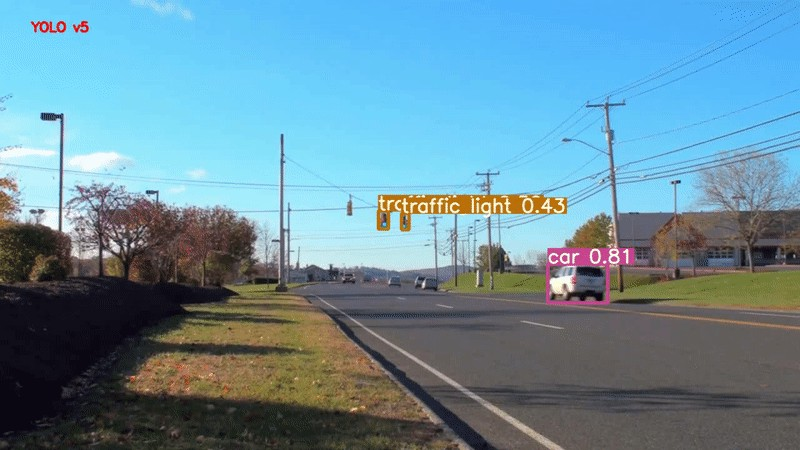
\includegraphics[scale=0.5]{img/who_wins_traffic_light_YOLO.jpg}
    \longcaption{YOLOv5 model in a driving video.}{YOLOv5 model in a driving video~\cite{Dwivedi2020YOLOv5}.}
    \label{fig:who_wins_traffic_light_YOLO}
\end{figure}

\begin{figure}[p]
    \centering
    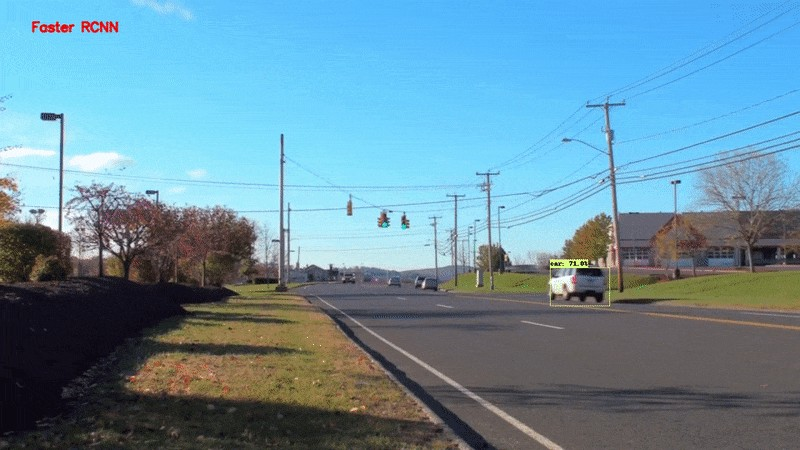
\includegraphics[scale=0.5]{img/who_wins_traffic_light_RCNN.jpg}
    \longcaption{Faster RCNN model in a driving video.}{Faster RCNN model in a driving video~\cite{Dwivedi2020YOLOv5}.}
    \label{fig:who_wins_traffic_light_RCNN}
\end{figure}

\begin{figure}[p]
    \centering
    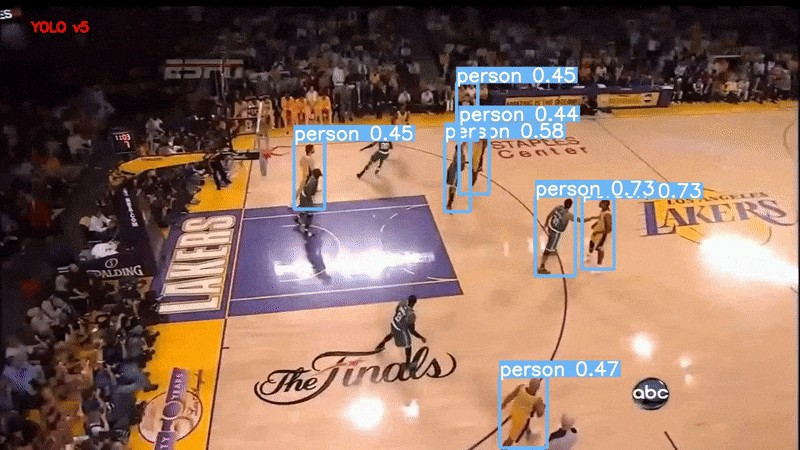
\includegraphics[scale=0.5]{img/who_wins_nba_YOLO.jpg}
    \longcaption{YOLOv5 model in an NBA game video.}{YOLOv5 model in an NBA game video~\cite{Dwivedi2020YOLOv5}.}
    \label{fig:who_wins_nba_YOLO}
\end{figure}

\begin{figure}[p]
    \centering
    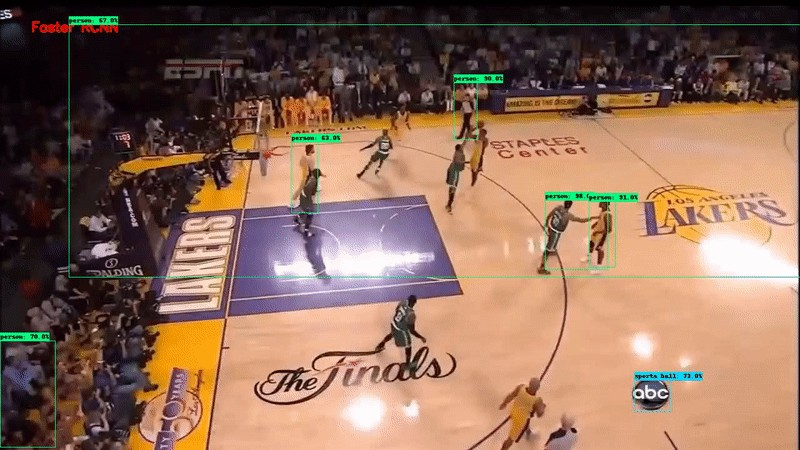
\includegraphics[scale=0.5]{img/who_wins_nba_RCNN.jpg}
    \longcaption{Faster RCNN model in an NBA game video.}{Faster RCNN model in an NBA game video~\cite{Dwivedi2020YOLOv5}.}
    \label{fig:who_wins_nba_RCNN}
\end{figure}


According to the official YOLOv5 tutorial, YOLOv5 has four different categories of models, YOLOv5s, YOLOv5m, YOLOv5l, and YOLOv5x. They have 7.3 million, 21.4 million, 47 million and 87.7 million parameters respectively. The official performance charts are also available, as shown in the Figure~\ref{fig:YOLOv5_Performance}.\\

\begin{figure}[h]
    \centering
    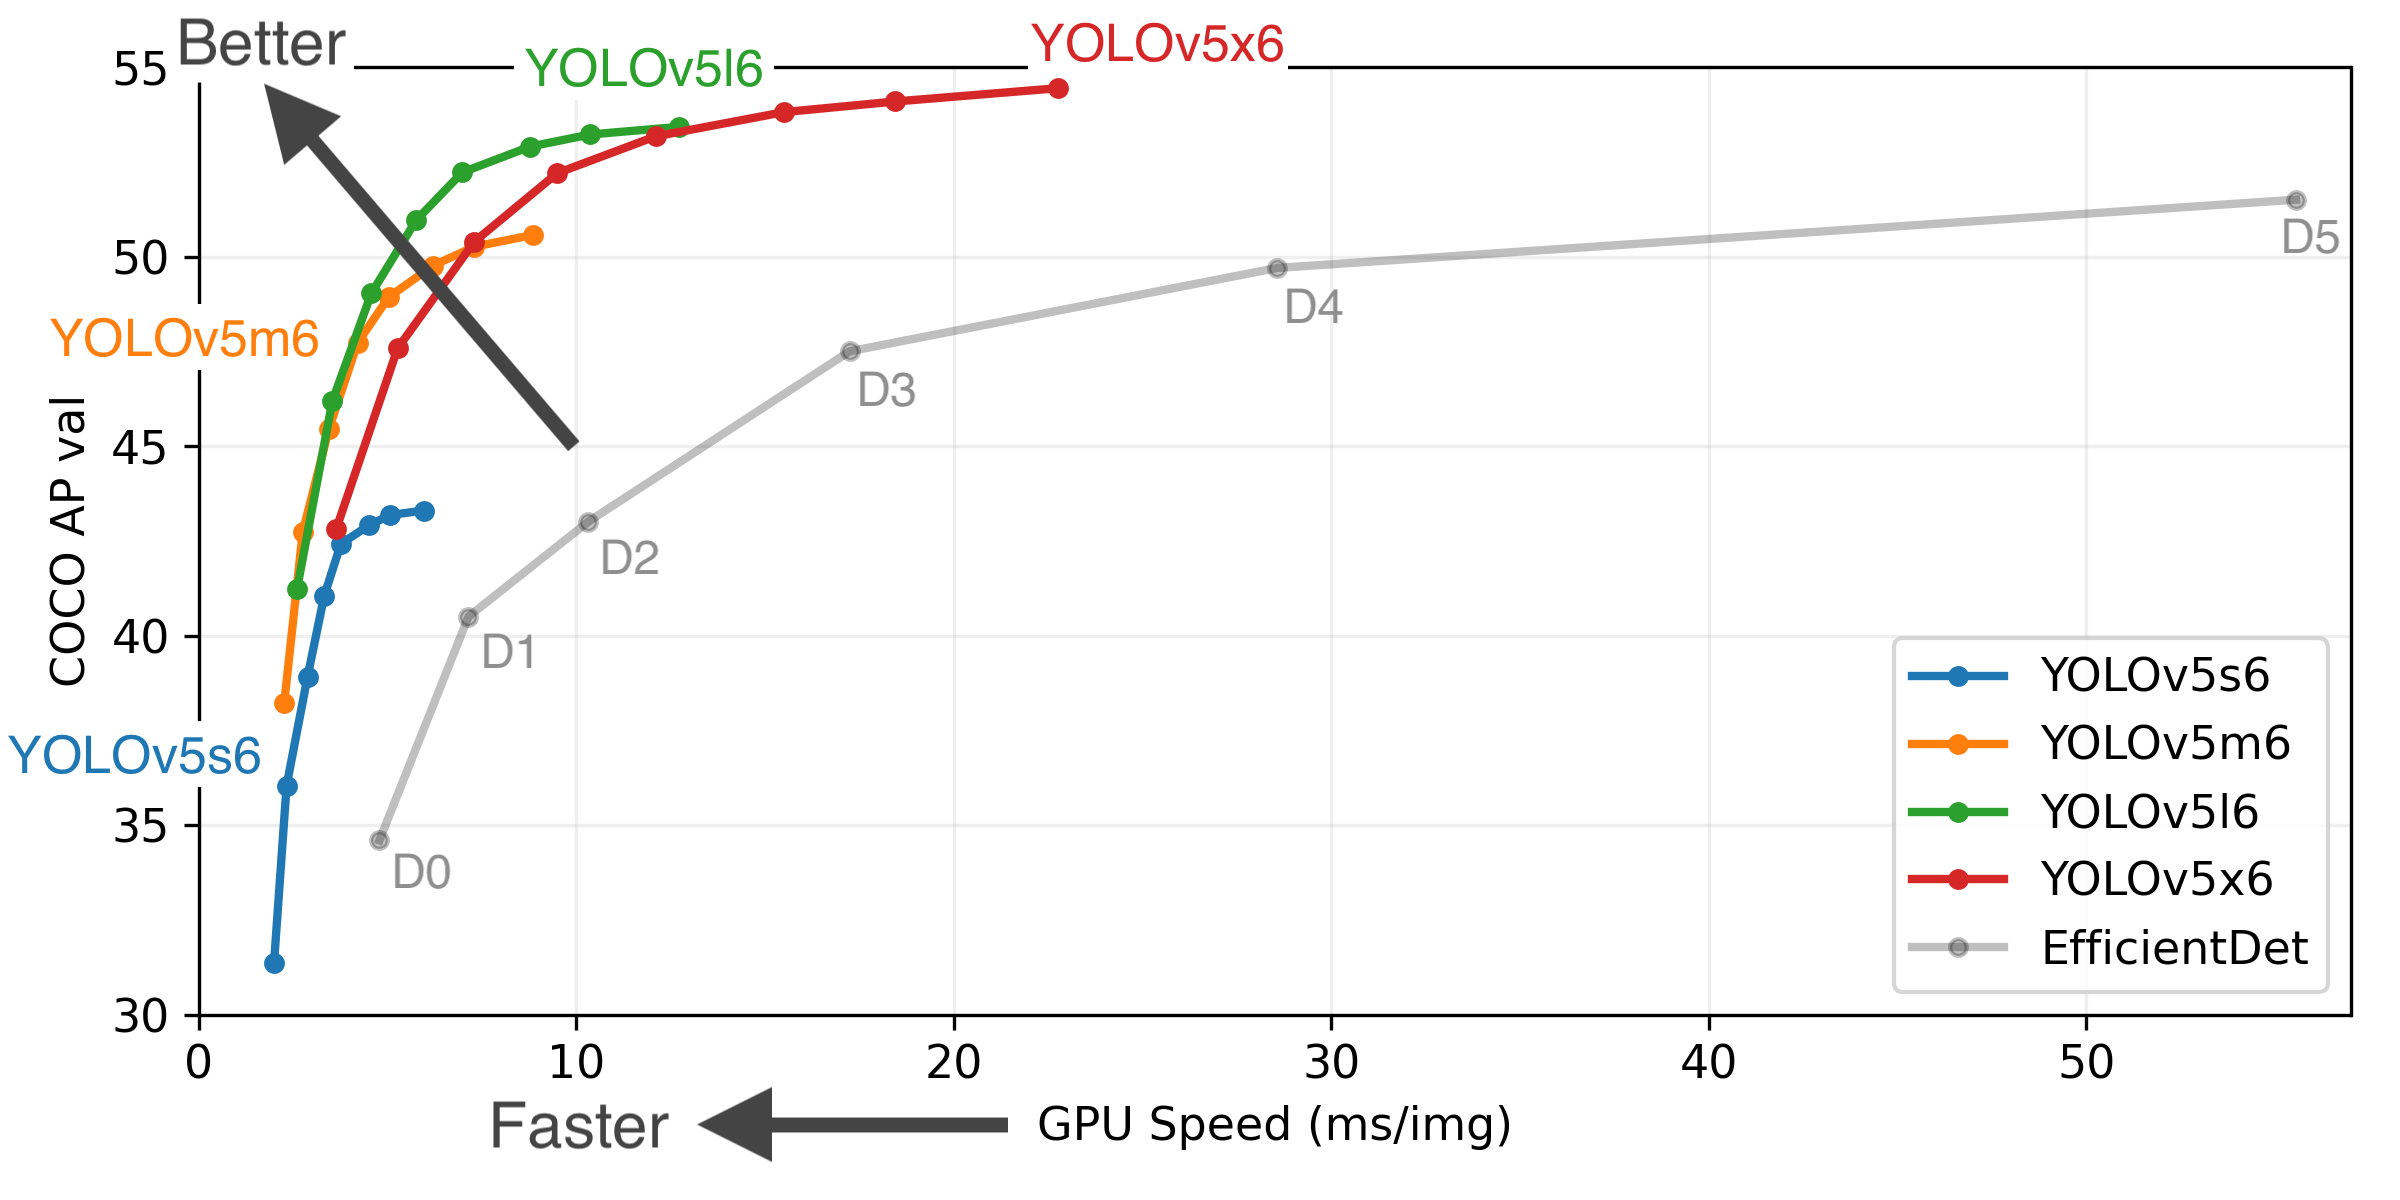
\includegraphics[scale=0.7]{img/YOLOv5_Performance.png}
    \longcaption{COCO Average Precision (AP) vs. GPU Speed in YOLOv5.}{COCO Average Precision (AP) vs. GPU Speed in YOLOv5~\cite{glenn_jocher_2020_4154370}.}
    \label{fig:YOLOv5_Performance}
\end{figure}

Thus, the YOLOv5l model is able to achieve higher average precision with the same faster computing speed. Thus, in this thesis, the YOLOv5l model was chosen as the model for the training dataset.\\



\newpage
\subsection{Data Source and Improvements}
Artificial intelligence algorithms need to be complemented by a large amount of data. An open-source data from a former TU Berlin researcher Tom Lutherborrow at Kaggle was used in this thesis. This open-source data contains 794 high-resolution images of ships from Google Earth~\cite{lutherborrowship}. However, this dataset is too much large than expected. Each image is larger than 9 megabytes, which is an efficiency burden for the training of neural networks, especially when there are few objects to be detected. With the tool RoboFlow, each training image can be resized to a 416x416 pixel image.\\


\subsection{Computing Power: CPU or GPU}
Another important foundation of artificial intelligence is computing power. For example, in this convolutional neural network algorithm that we have just done, each calculation is actually not very complicated: it is just addition and multiplication. But the amount of computation is huge. For instance, there is an image that is 800x600, but due to the RGB colours, there are around 1.44 million pixels in total. Using a 3x3x3 convolution kernel will take about 13 million multiplications and about 12 million additions. It's simple addition and multiplication, but it's a vast number of operations. Besides, that's just using a convolution kernel for a simple image. There are actually thousands of images convolved thousands of times during the training process, so that's a vast number of operations.\\

The GPU was originally meant to be a graphics processing unit, and it has a parallel structure that allows for more efficient computing than a central processing unit (CPU). For instance, if a link in a neural network is being computed simultaneously with another link, a large number of small cores can be used simultaneously to speed up the computation. In this thesis, all ConvNet models were trained using a YOLOv5 framework with Tesla P100 GPU in the Google Colab.\\




\section{Algorithms for Detection and Classification}
\subsection{Target Areas in the Gulf of California}
\label{sec3.2.1}
The Gulf of Californian was chosen as an area of study for this thesis. Ideally, in order to analyse a sufficient amount of satellite image data, the ports of each of the major harbour cities in the Gulf of California would need to be included in the scope of our study. Thus, it was worth to finding out if there was enough data for the area in Google Earth Pro. The results of the statistics can be seen in Table~\ref{table:baja_california_dates}, Table~\ref{table:Baja_California_Sur_dates}, Table~\ref{table:Sonora_dates}, Table~\ref{table:Sinaloa_dates}, Table~\ref{table:Nayarit_dates}, Table~\ref{table:Jalisco_dates}, Table~\ref{table:Colima_dates}.\\

In fact, Google Earth Pro provided very little image data than was expected. Most of the Mexican cities in the Gulf of California do not have satellite data for 2021. A few cities have satellite data from 2018. More cities have satellite data for 2019 and 2020. This reflects that:
\begin{itemize}
    \item a steady increase in the collection of satellite data in the Gulf of California.
    \item that the free, high-quality satellite data available from Google Earth Pro is not immediately available for publication.
    \item regional differences in satellite data are still evident. Some cities, such as Guaymas, will have access to about 15 satellite images a year in 2019 or 2020. However, some cities, such as La Ventana, did not appear in Google Earth Pro in 2019 and 2020, when almost all other cities have been photographed by satellite.\\
\end{itemize}

For this reason, it is clear that continuing with the previous strategy of analysing the satellite data for each city in the Gulf of California (from Table~\ref{table:baja_california_dates} to Table~\ref{table:Jalisco_dates}) would lead to a relatively large information bias and thus would not achieve an accurate result of the composition of the boats of the Gulf of California. Therefore, the following three cities with the most data in Google Earth Pro were finally chosen as the target areas for this thesis: Santa Rosalia, Loreto, Guaymas.\\

% Table 3.1
\begin{table}[h!]
\centering
\begin{tabular}{ l | p{2.5cm} | p{2.5cm} | p{2.5cm} | p{2.5cm} }
\toprule
City & 2021 & 2020 & 2019 & 2018 \\
\midrule
San Felipe & NA & 12/30; 12/26; 12/9; 11/17; 11/1; 4/19 & 6/17; 2/5; 1/22 & 10/23; 9/29; 3/3; 3/1; 2/26; 2/5\\
\midrule
Bahia de los Angeles & NA & 5/15 & 6/17 & 11/10\\
\midrule
Isla Smith & NA & NA & 6/17 & NA\\
\bottomrule
\end{tabular}
\caption{Specific dates when Google Earth Pro has images from 2018 to 2021 in Baja California, Meico.}
\label{table:baja_california_dates}
\end{table}


% Table 3.4
\begin{table}[h!]
\centering
\begin{tabular}{ l | p{2.5cm} | p{2.5cm} | p{2.5cm} | p{2.5cm} }
\toprule
City & 2021 & 2020 & 2019 & 2018 \\
\midrule
Los Mochis & 2/1; 1/31 & 12/2; 9/30; 9/15; 9/12; 4/20; 1/29; 1/18 & 12/8; 8/3; 7/12; 6/13; 4/30; 2/7 & 11/6; 10/20; 7/3\\
\midrule
La Cruz & 1/16 & 10/31; 2/25; 2/21 & 10/29; 8/1; 7/10; 6/20; 4/19; 1/27 & 11/3; 10/16; 8/9; 1/17\\
\midrule
Mazatlan & NA & 10/31; 10/1; 9/19; 9/10; 8/29; 7/21; 2/28; 1/26; 1/18 & 12/7; 11/30; 8/3 & 11/3; 10/30; 10/27; 10/24; 10/12; 8/4; 6/27; 5/11; 4/19; 1/12\\
\bottomrule
\end{tabular}
\caption{Specific dates when Google Earth Pro has images from 2018 to 2021 in Sinaloa, Meico.}
\label{table:Sinaloa_dates}
\end{table}

% Table 3.7
\begin{table}[h!]
\centering
\begin{tabular}{ l | p{2.5cm} | p{2.5cm} | p{2.5cm} | p{2.5cm} }
\toprule
City & 2021 & 2020 & 2019 & 2018 \\
\midrule
Manzanillo & NA & 12/26; 9/14; 5/31; 3/3; 1/12 & 12/9; 3/7; 3/6 & NA\\
\bottomrule
\end{tabular}
\caption{Specific dates when Google Earth Pro has images from 2018 to 2021 in Colima, Meico.}
\label{table:Colima_dates}
\end{table}


% Table 3.2
\begin{table}[p]
\centering
\begin{tabular}{ l | p{2.5cm} | p{2.5cm} | p{2.5cm} | p{2.5cm} }
\toprule
City & 2021 & 2020 & 2019 & 2018 \\
\midrule
Santa Rosalia & NA & 12/21; 12/9; 11/28; 11/1; 9/11; 8/11; 8/6; 7/17; 7/14; 7/10; 7/6; 6/22; 6/17; 6/9; 5/26; 5/18; 5/8; 4/26; 4/18; 4/14; 3/15; 2/14; 2/3; 1/28; 1/27; 1/22; 1/13; 1/5 & 12/19; 12/14; 12/11; 12/3; 10/31; 10/20; 9/24; 9/20; 9/9; 8/26; 8/21; 8/11; 7/8; 7/5; 4/17; 1/30 & 11/9; 7/4; 6/7; 4/2; 2/23\\
\midrule
Mulege & 1/18 & NA & 7/8 & NA\\
\midrule
Loreto & 2/12; 1/18 & 11/25; 11/23; 11/22; 11/4; 9/26; 9.13; 8/25; 8/17; 8/14; 7/29; 7/25; 7/16; 7/14; 7/10; 6/25; 6/3; 4/30; 4/23; 4/22; 4/18; 4/11; 3/16; 2/25; 1/29; 1/18; 1/2 & 12/30; 12/11; 11/1; 10/31; 10/7; 10/4; 9/26; 8/27; 8/26; 8/19; 7/9; 6/22; 4/26; 4/11; 1/30 & 10/2; 9/26; 8/14\\
\midrule
La Paz & NA & 1/18 & NA & 4/4\\
\midrule
La Ventana & NA & NA & NA & 4/4\\
\midrule
San Jose del Cabo & NA & NA & NA & 3/28\\
\midrule
Cabo San Lucas & NA & 3/28 & NA & 3/28\\
\bottomrule
\end{tabular}
\caption{Specific dates when Google Earth Pro has images from 2018 to 2021 in Baja California Sur, Meico.}
\label{table:Baja_California_Sur_dates}
\end{table}


% Table 3.3
\begin{table}[p]
\centering
\begin{tabular}{ l | p{2.5cm} | p{2.5cm} | p{2.5cm} | p{2.5cm} }
\toprule
City & 2021 & 2020 & 2019 & 2018 \\
\midrule
Golfo de Santa Clara & 1/9 & NA & 6/24 & NA\\
\midrule
Puerto Penasco & 1/26 & 8/27; 8/19; 7/28; 2/15 & 11/30; 11/7; 10/15; 10/12; 10/1; 6/19; 6/17; 2/15; 2/12; 2/7; 1/27; 1/25 & 10/10; 9/29; 9/13\\
\midrule
Bahia de Kino & 1/10 & NA & 6/25; 6/18 & NA\\
\midrule
Guaymas & 2/10 & 12/9; 11/28; 11/9; 10/24; 9/24; 8/23; 8/17; 8/9; 7/26; 7/10; 5/27; 5/13; 4/23; 4/14; 3/6; 2/6; 2/1; 1/29; 1/7 & 11/13; 11/1; 9/15; 7/15; 6/21; 6/20; 6/13; 6/9; 4/24; 4/19; 3/9; 2/4; 1/19 & 11/1; 7/20; 3/16; 1/22\\
\bottomrule
\end{tabular}
\caption{Specific dates when Google Earth Pro has images from 2018 to 2021 in Sonora, Meico.}
\label{table:Sonora_dates}
\end{table}


% Table 3.5
\begin{table}[p]
\centering
\begin{tabular}{ l | p{2.5cm} | p{2.5cm} | p{2.5cm} | p{2.5cm} }
\toprule
City & 2021 & 2020 & 2019 & 2018 \\
\midrule
San Blas & NA & 1/6 & 2/27 & 10/11; 5/7; 4/10; 2/27\\
\bottomrule
\end{tabular}
\caption{Specific dates when Google Earth Pro has images from 2018 to 2021 in Nayarit, Meico.}
\label{table:Nayarit_dates}
\end{table}


% Table 3.6
\begin{table}[p]
\centering
\begin{tabular}{ l | p{2.5cm} | p{2.5cm} | p{2.5cm} | p{2.5cm} }
\toprule
City & 2021 & 2020 & 2019 & 2018 \\
\midrule
Puerto Vallarta & NA & 5/1; 3/28 & NA & 3/27; 3/21; 3/19\\
\bottomrule
\end{tabular}
\caption{Specific dates when Google Earth Pro has images from 2018 to 2021 in Jalisco, Meico.}
\label{table:Jalisco_dates}
\end{table}



\subsection{Image Kernel and Image Sharpening}
\label{sec3.2.2}
Similar to the principle of using convolution kernels, specific image kernels can sharpen the image. While the sharpening kernel does not make the image higher resolution, it emphasises the differences in adjacent pixel values which makes the image look more vivid. Overall, with the same model weight, as shown in Figure~\ref{fig:sharpening}, sharpening an image can significantly improve the recognition accuracy of an image with a 5x5 image kernel.\\

\begin{figure}[h!]
\centering
\begin{subfigure}[p]{0.7\textwidth}
    \centering
    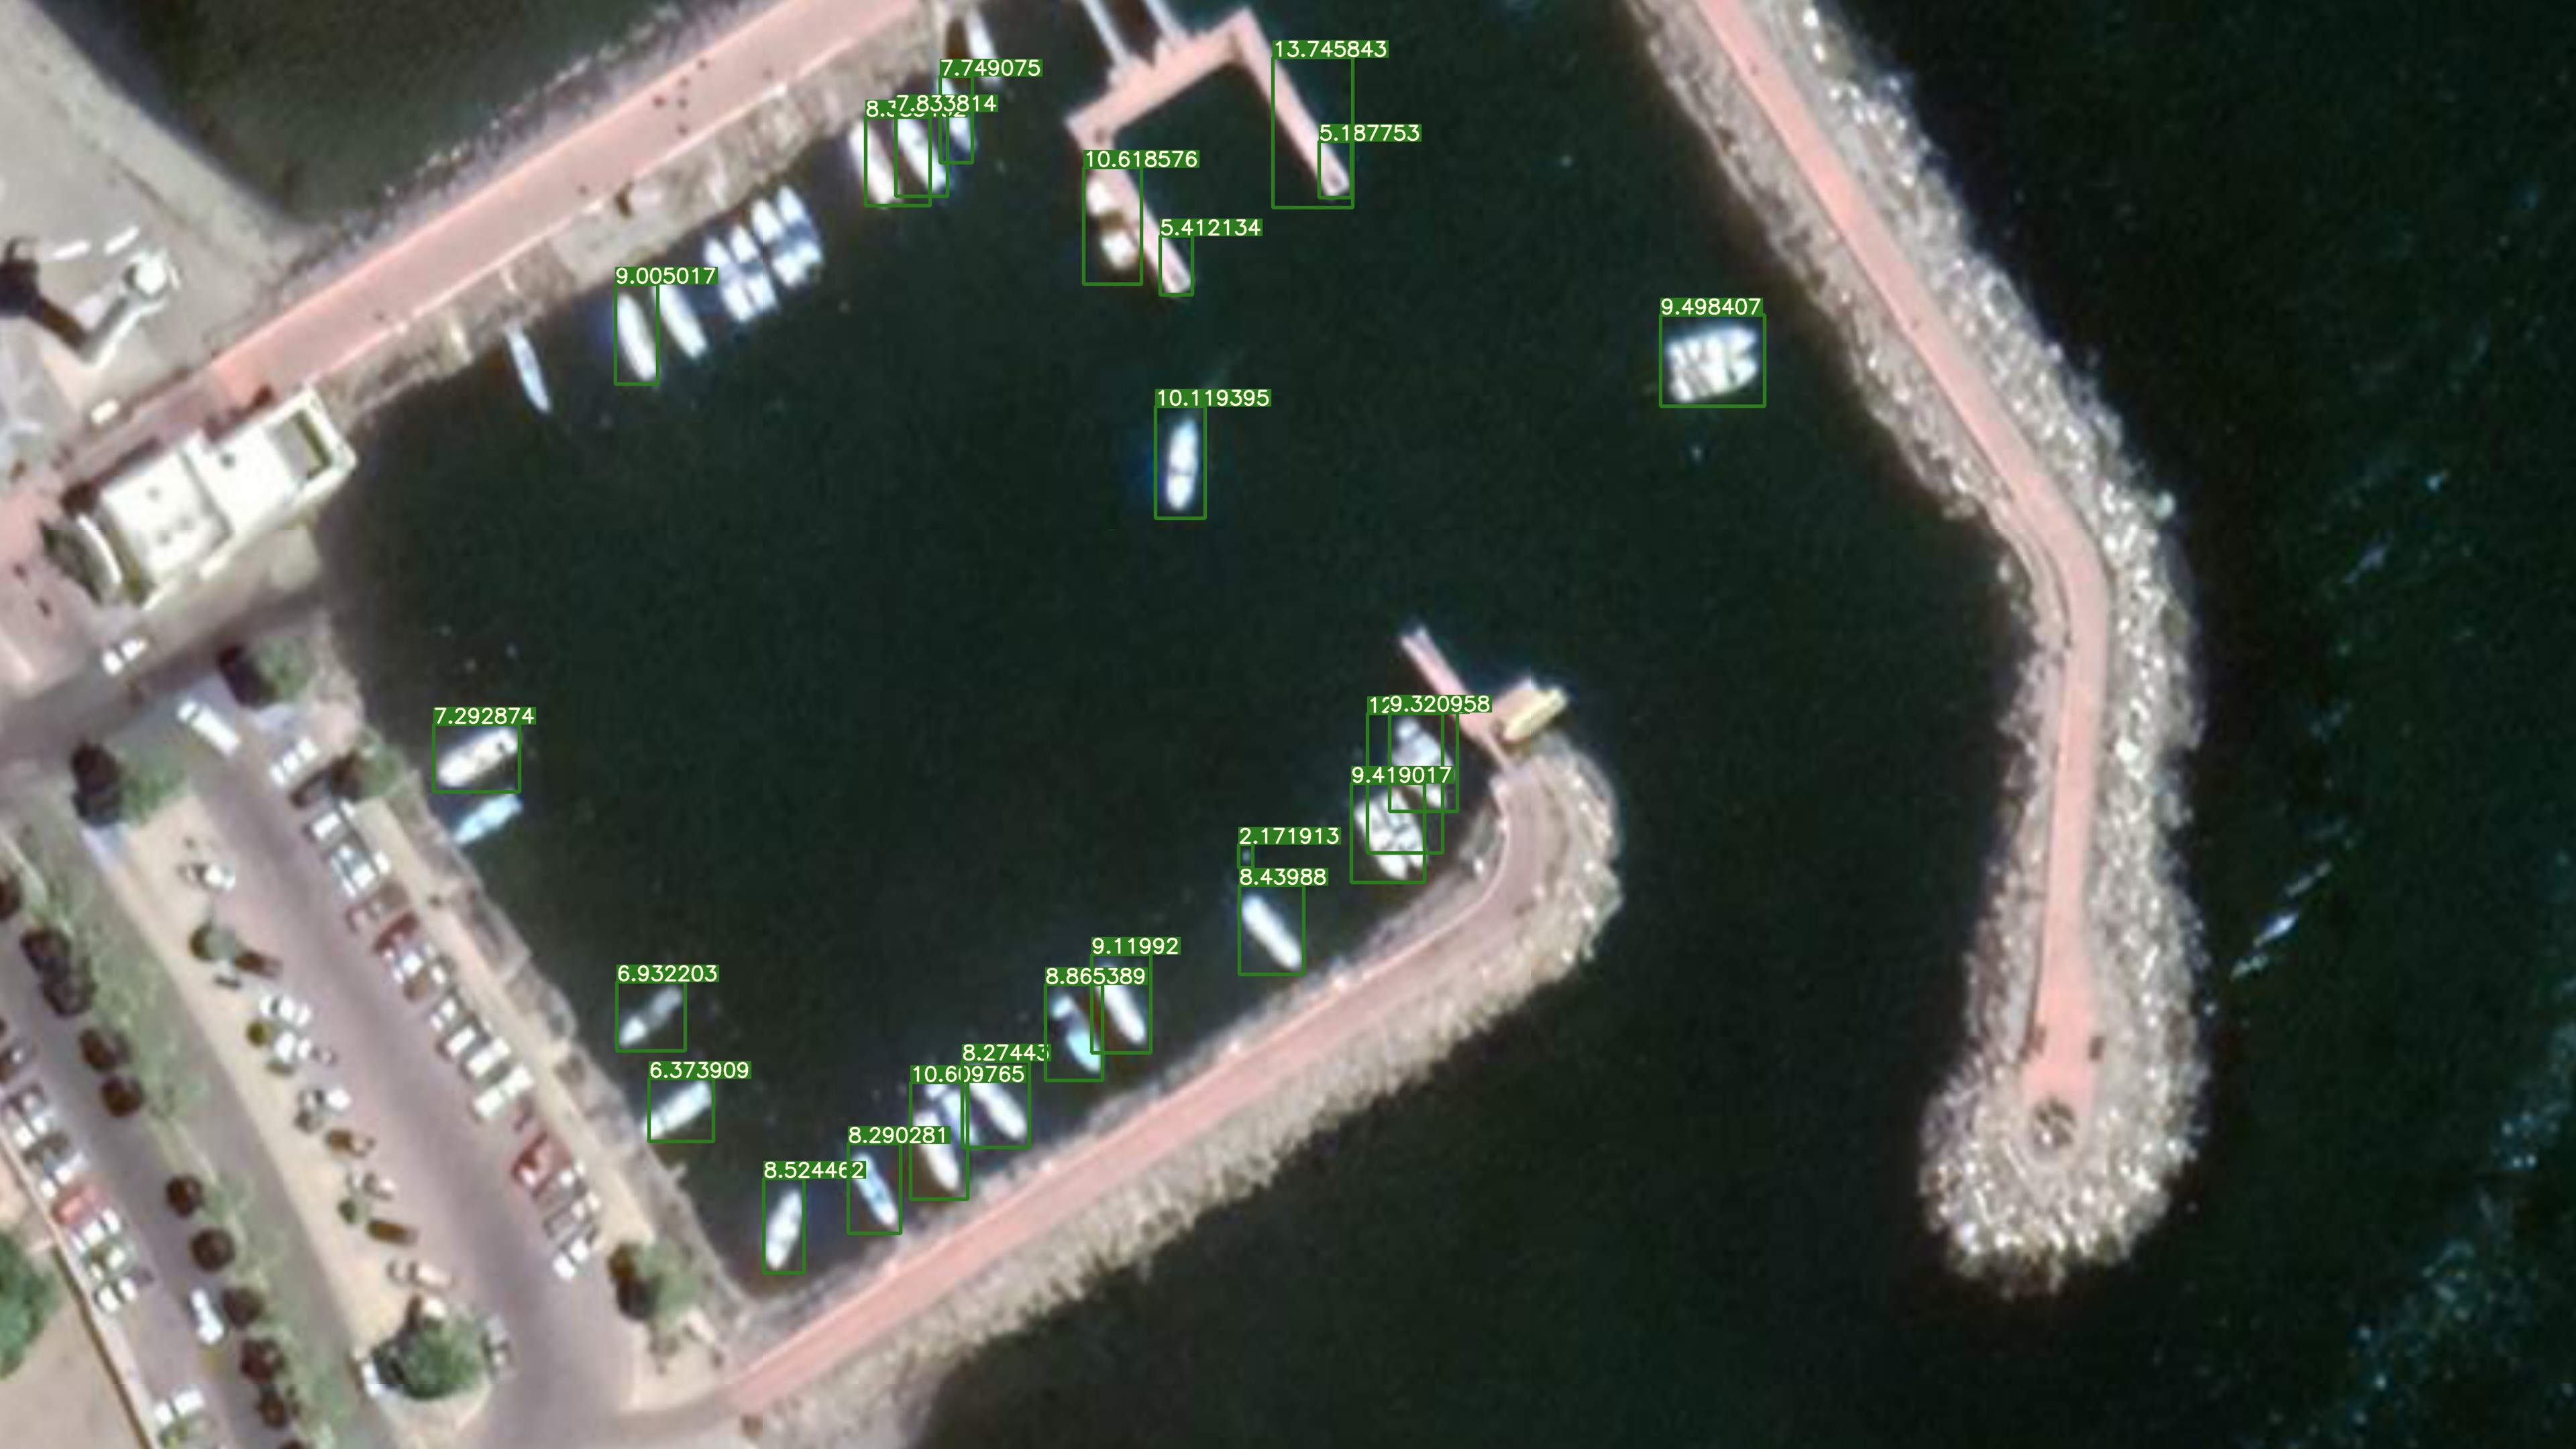
\includegraphics[width=1\linewidth]{img/before_sharpening.jpg}
    \caption{Detection before sharpening.}
    \label{fig:before_sharpening}
\end{subfigure}

\begin{subfigure}[p]{0.7\textwidth}
    \centering
    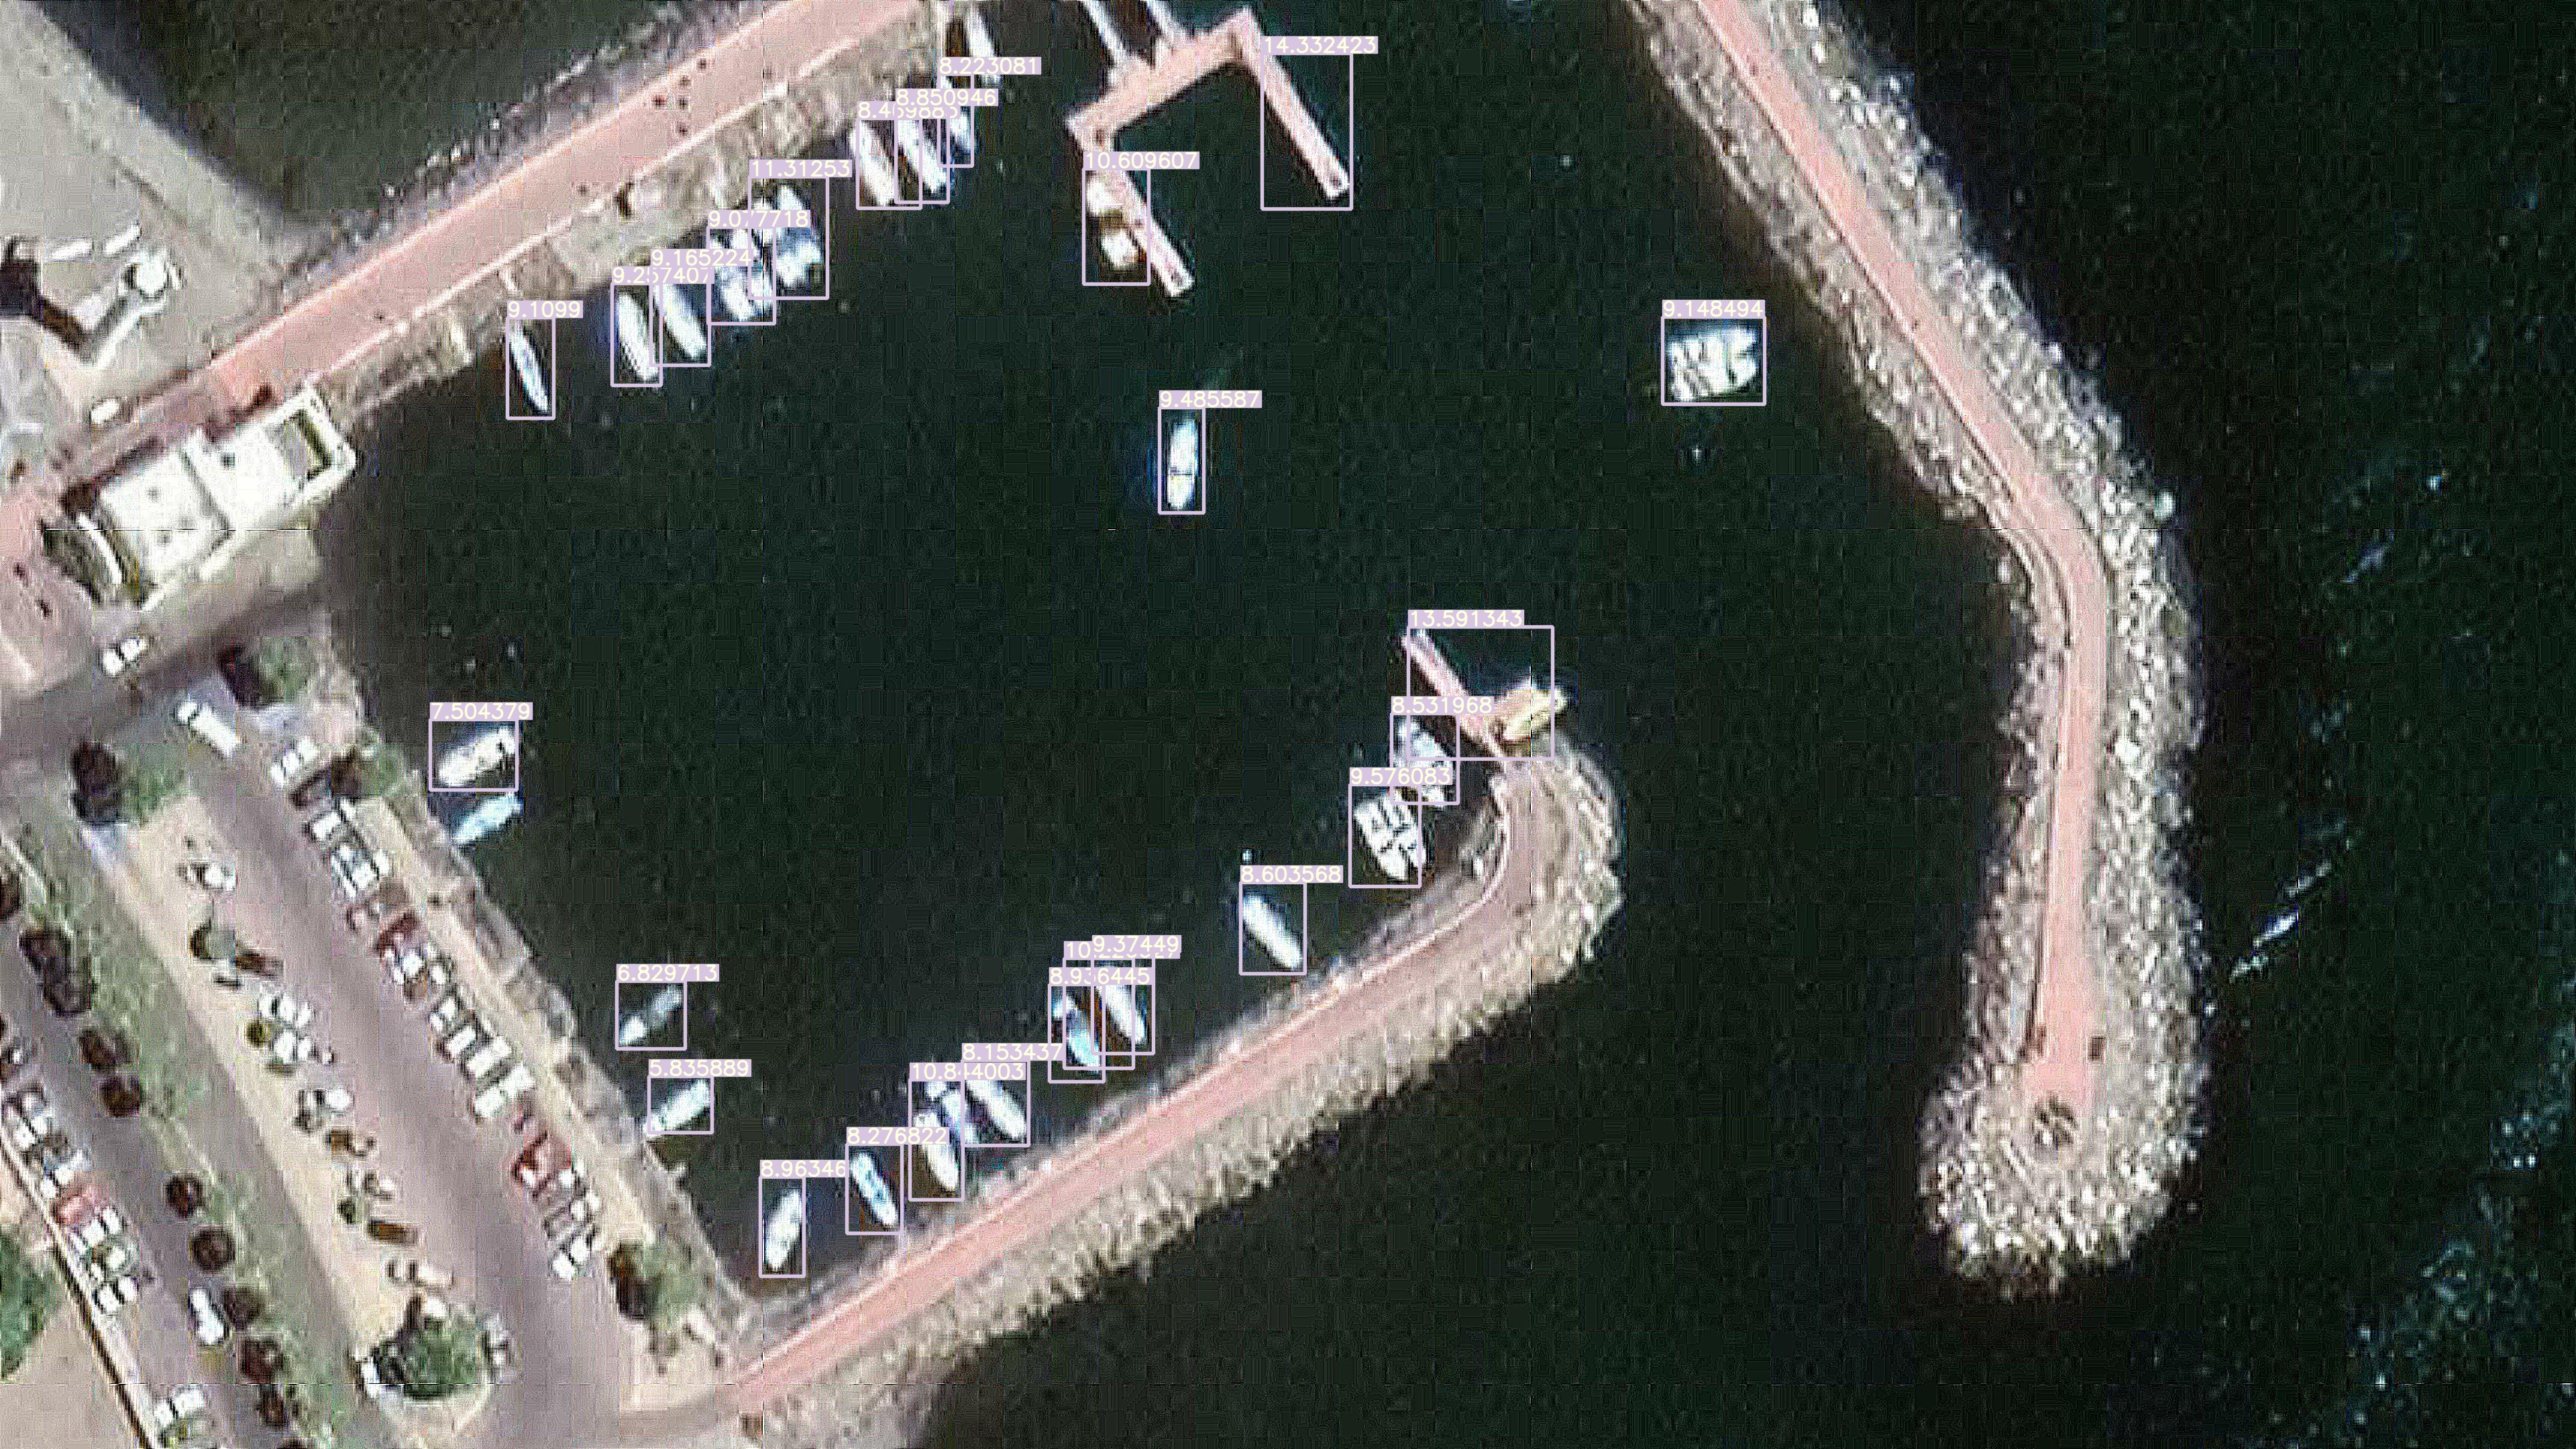
\includegraphics[width=1\linewidth]{img/after_sharpening.jpg}
    \caption{Detection after sharpening.}
    \label{fig:after_sharpening}
\end{subfigure}
\caption{Detections before and after sharpening}
\label{fig:sharpening}
\end{figure}


\newpage
\subsection{Detecting the Length of Small boats}
\label{sec3.2.3}
Measuring the length of a ship is one of the most difficult topics in this thesis. As Google Earth Pro does not provide an application programming interface (API) for accurate scales, manually measuring the size of a particular scale became the core of measuring the size of a ship.\\

As the dataset for the training model was created with each edge tangent to the edge of the detected object, we can roughly treat the boat's length as the length of the diagonal of the detection box. Secondly, since the scale is central to the production of the bay dataset that follows, i.e., the satellite image at this scale:
\begin{itemize}
    \item cannot be too large: they need to contain the full complement of small boats (if any), and the complexity of producing the dataset must also be considered.
    \item cannot be too small: otherwise, there is a tendency for multiple small boats docked together to be detected as a whole party.
    \item be sufficiently clear: the model needs to be allowed to accurately identify the length of small boats to reduce errors in scale.
\end{itemize}

Based on the above rules, the eye altitude was finally determined to be 200m. Meanwhile, I used a satellite image of Zurich Lake, Switzerland, on 16 August 2018 as the standard image for defining the scale (Figure~\ref{fig:zurich}). \\

After metering, the vessel in Figure~\ref{fig:zurich} with a YOLO length of 0.434517 is actually 55.17m. Then, with an eye altitude of 200 metres, the ratio of the real length to the YOLO length is approximately 127. Finally, after several verifications, this ratio is within the margin of error and can be used as a scaling ratio. And having the same ratio and the same eye altitude is not enough. We also need to keep the resolution of each image the same as well. For this purpose, all datasets involved in the detection will maintain a resolution of 3840x2160.\\

\begin{figure}
    \centering
    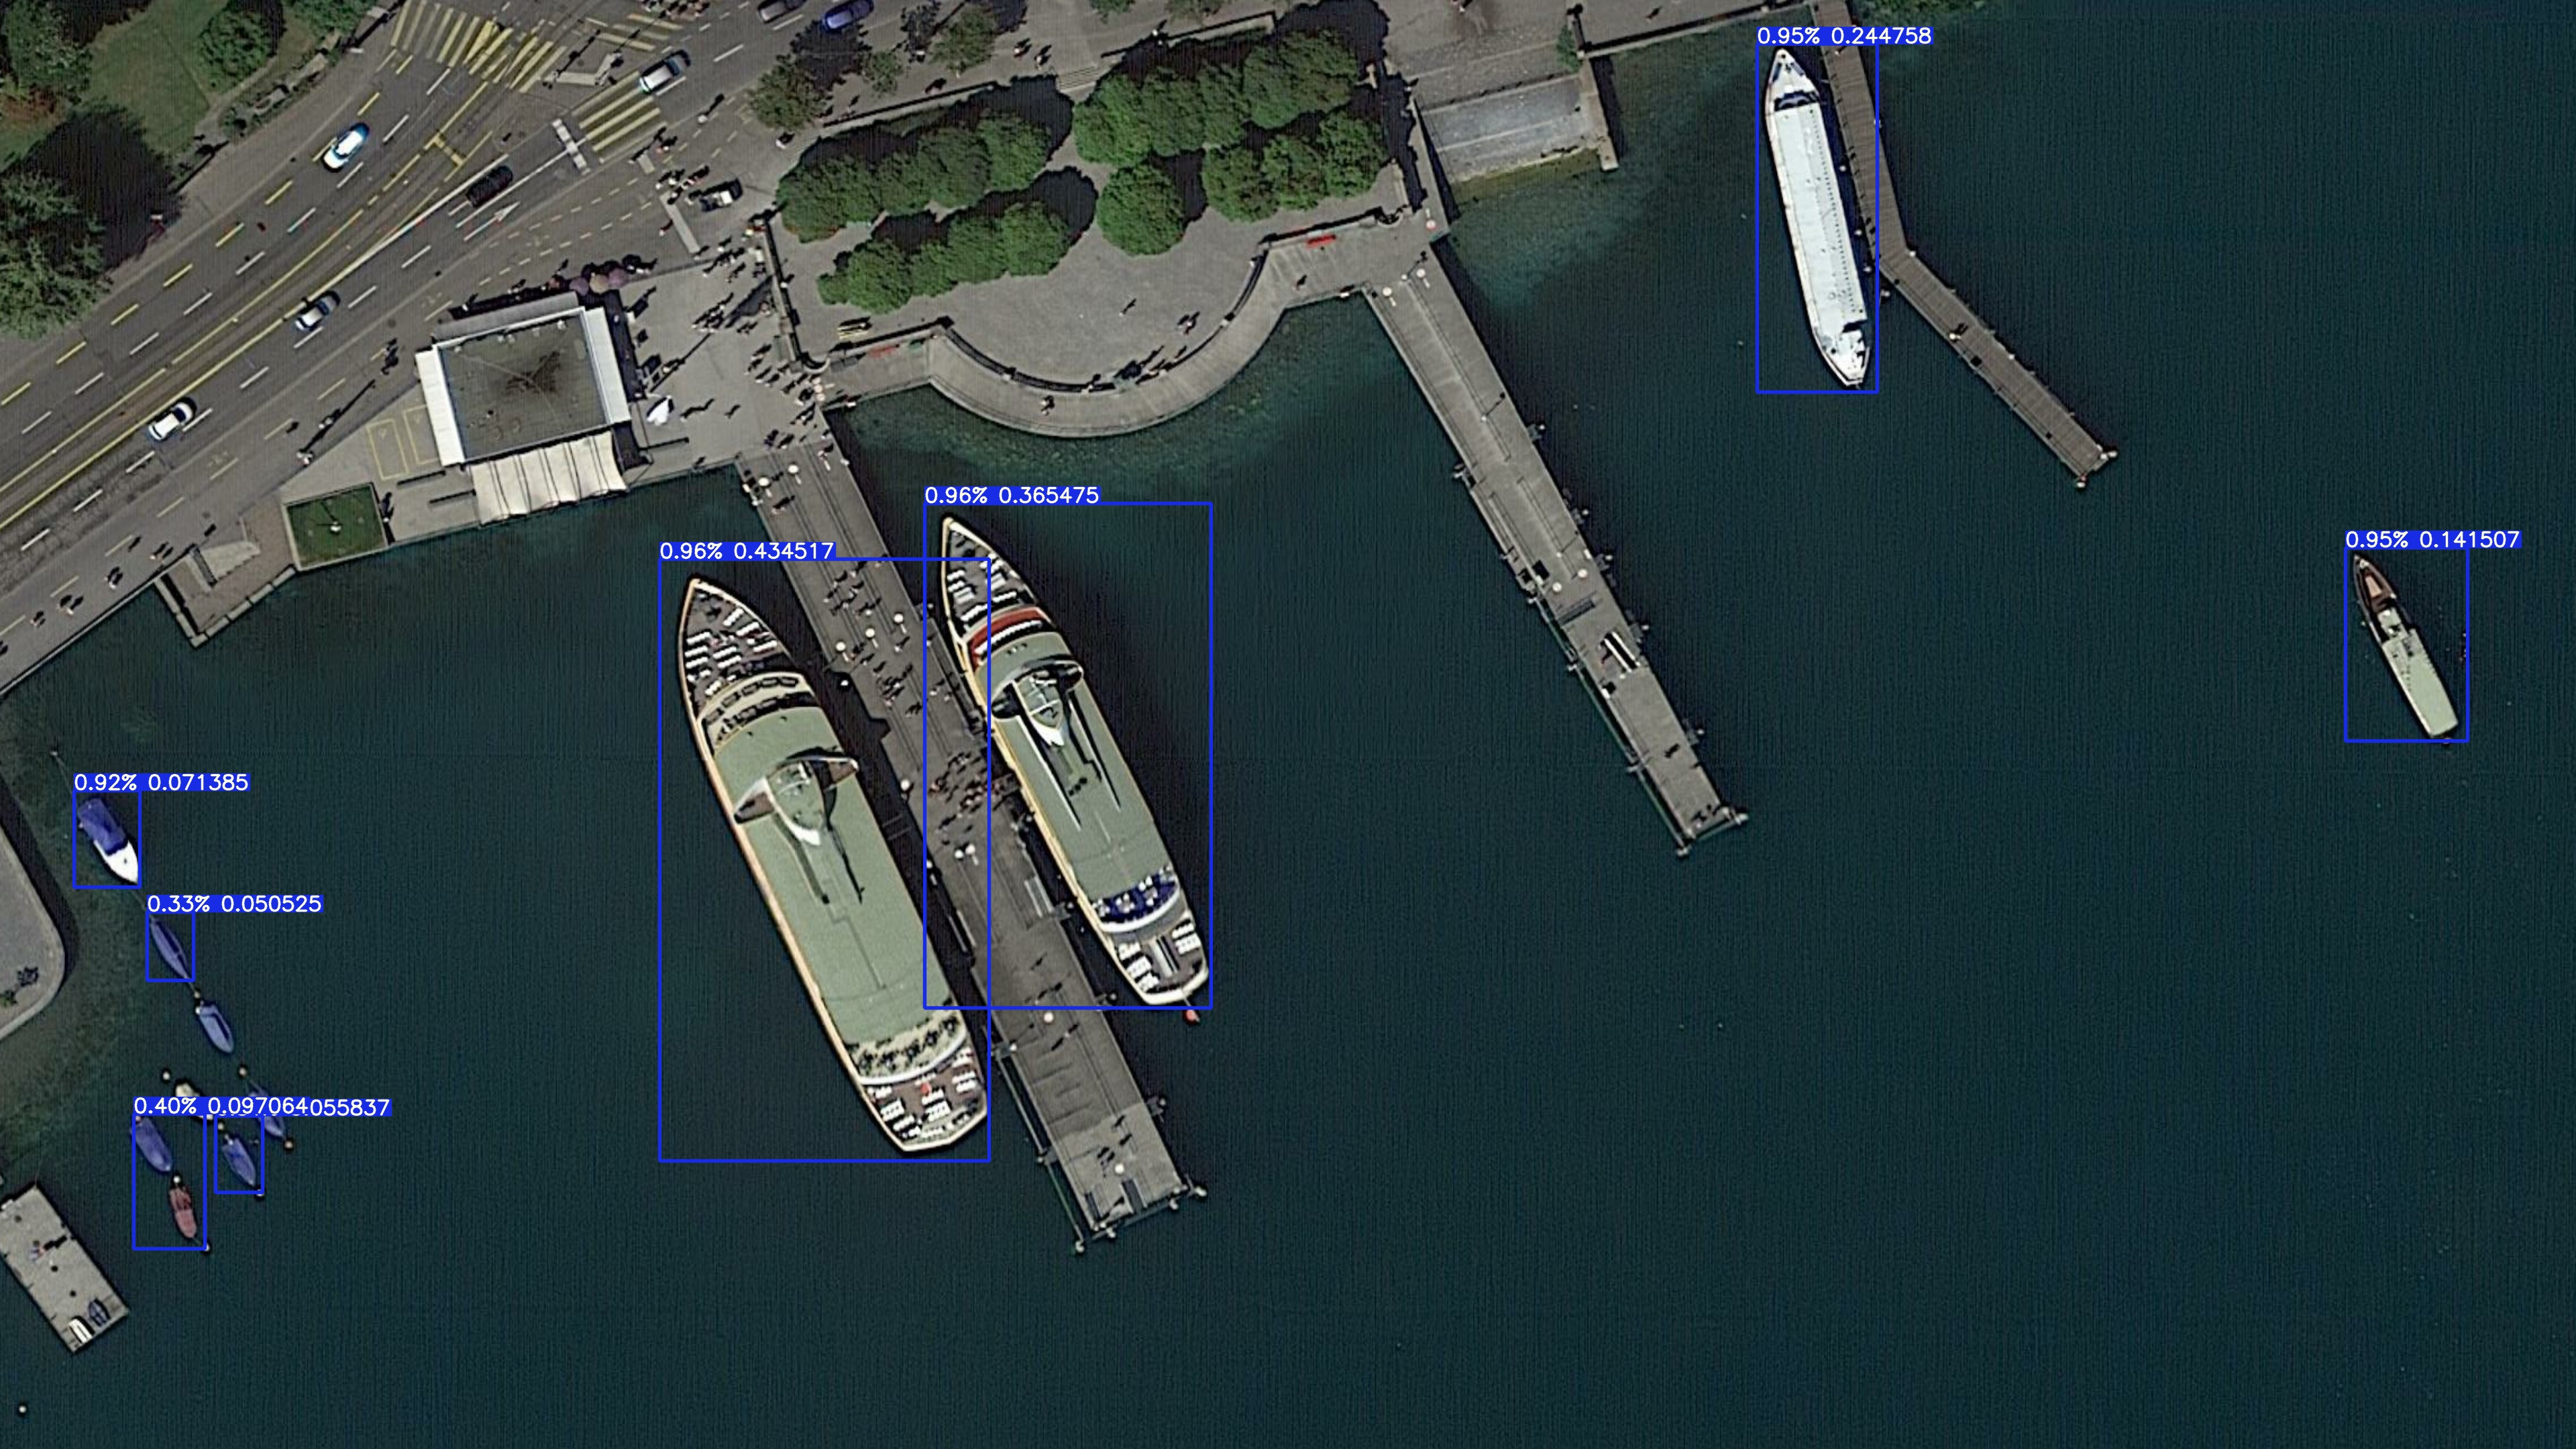
\includegraphics[scale=0.1]{img/zurich.jpg}
    \caption{An image from Google Earth Pro for Zurich Lake on 16 Aug 2018 when eye alt is 200 meters.}
    \label{fig:zurich}
\end{figure}


\newpage
\subsection{Classification of Small Boats and Big Boats}
In a certain sense, large vessels (e.g. cargo ships or warships) and small vessels (e.g. small boats for domestic use for recreation and fishing) are distinguished when creating the dataset for the area. However, due to the scaling, the eye altitude of the image is only 200 meters. Therefore, some enormous vessels, such as cargo ships, do not even appear fully in an image with a resolution of 3840x2160 (such as Figure~\ref{fig:Guaymas_202103_overflow_screen}), i.e., they do not appear in the statistical results. On the other hand, some of the larger vessels, slightly shorter in length, are identified correctly by the algorithm and counted as part of the number of large vessels in the area (Figure~\ref{fig:Guaymas_202105_detect_small_large}).

\begin{figure}
    \centering
    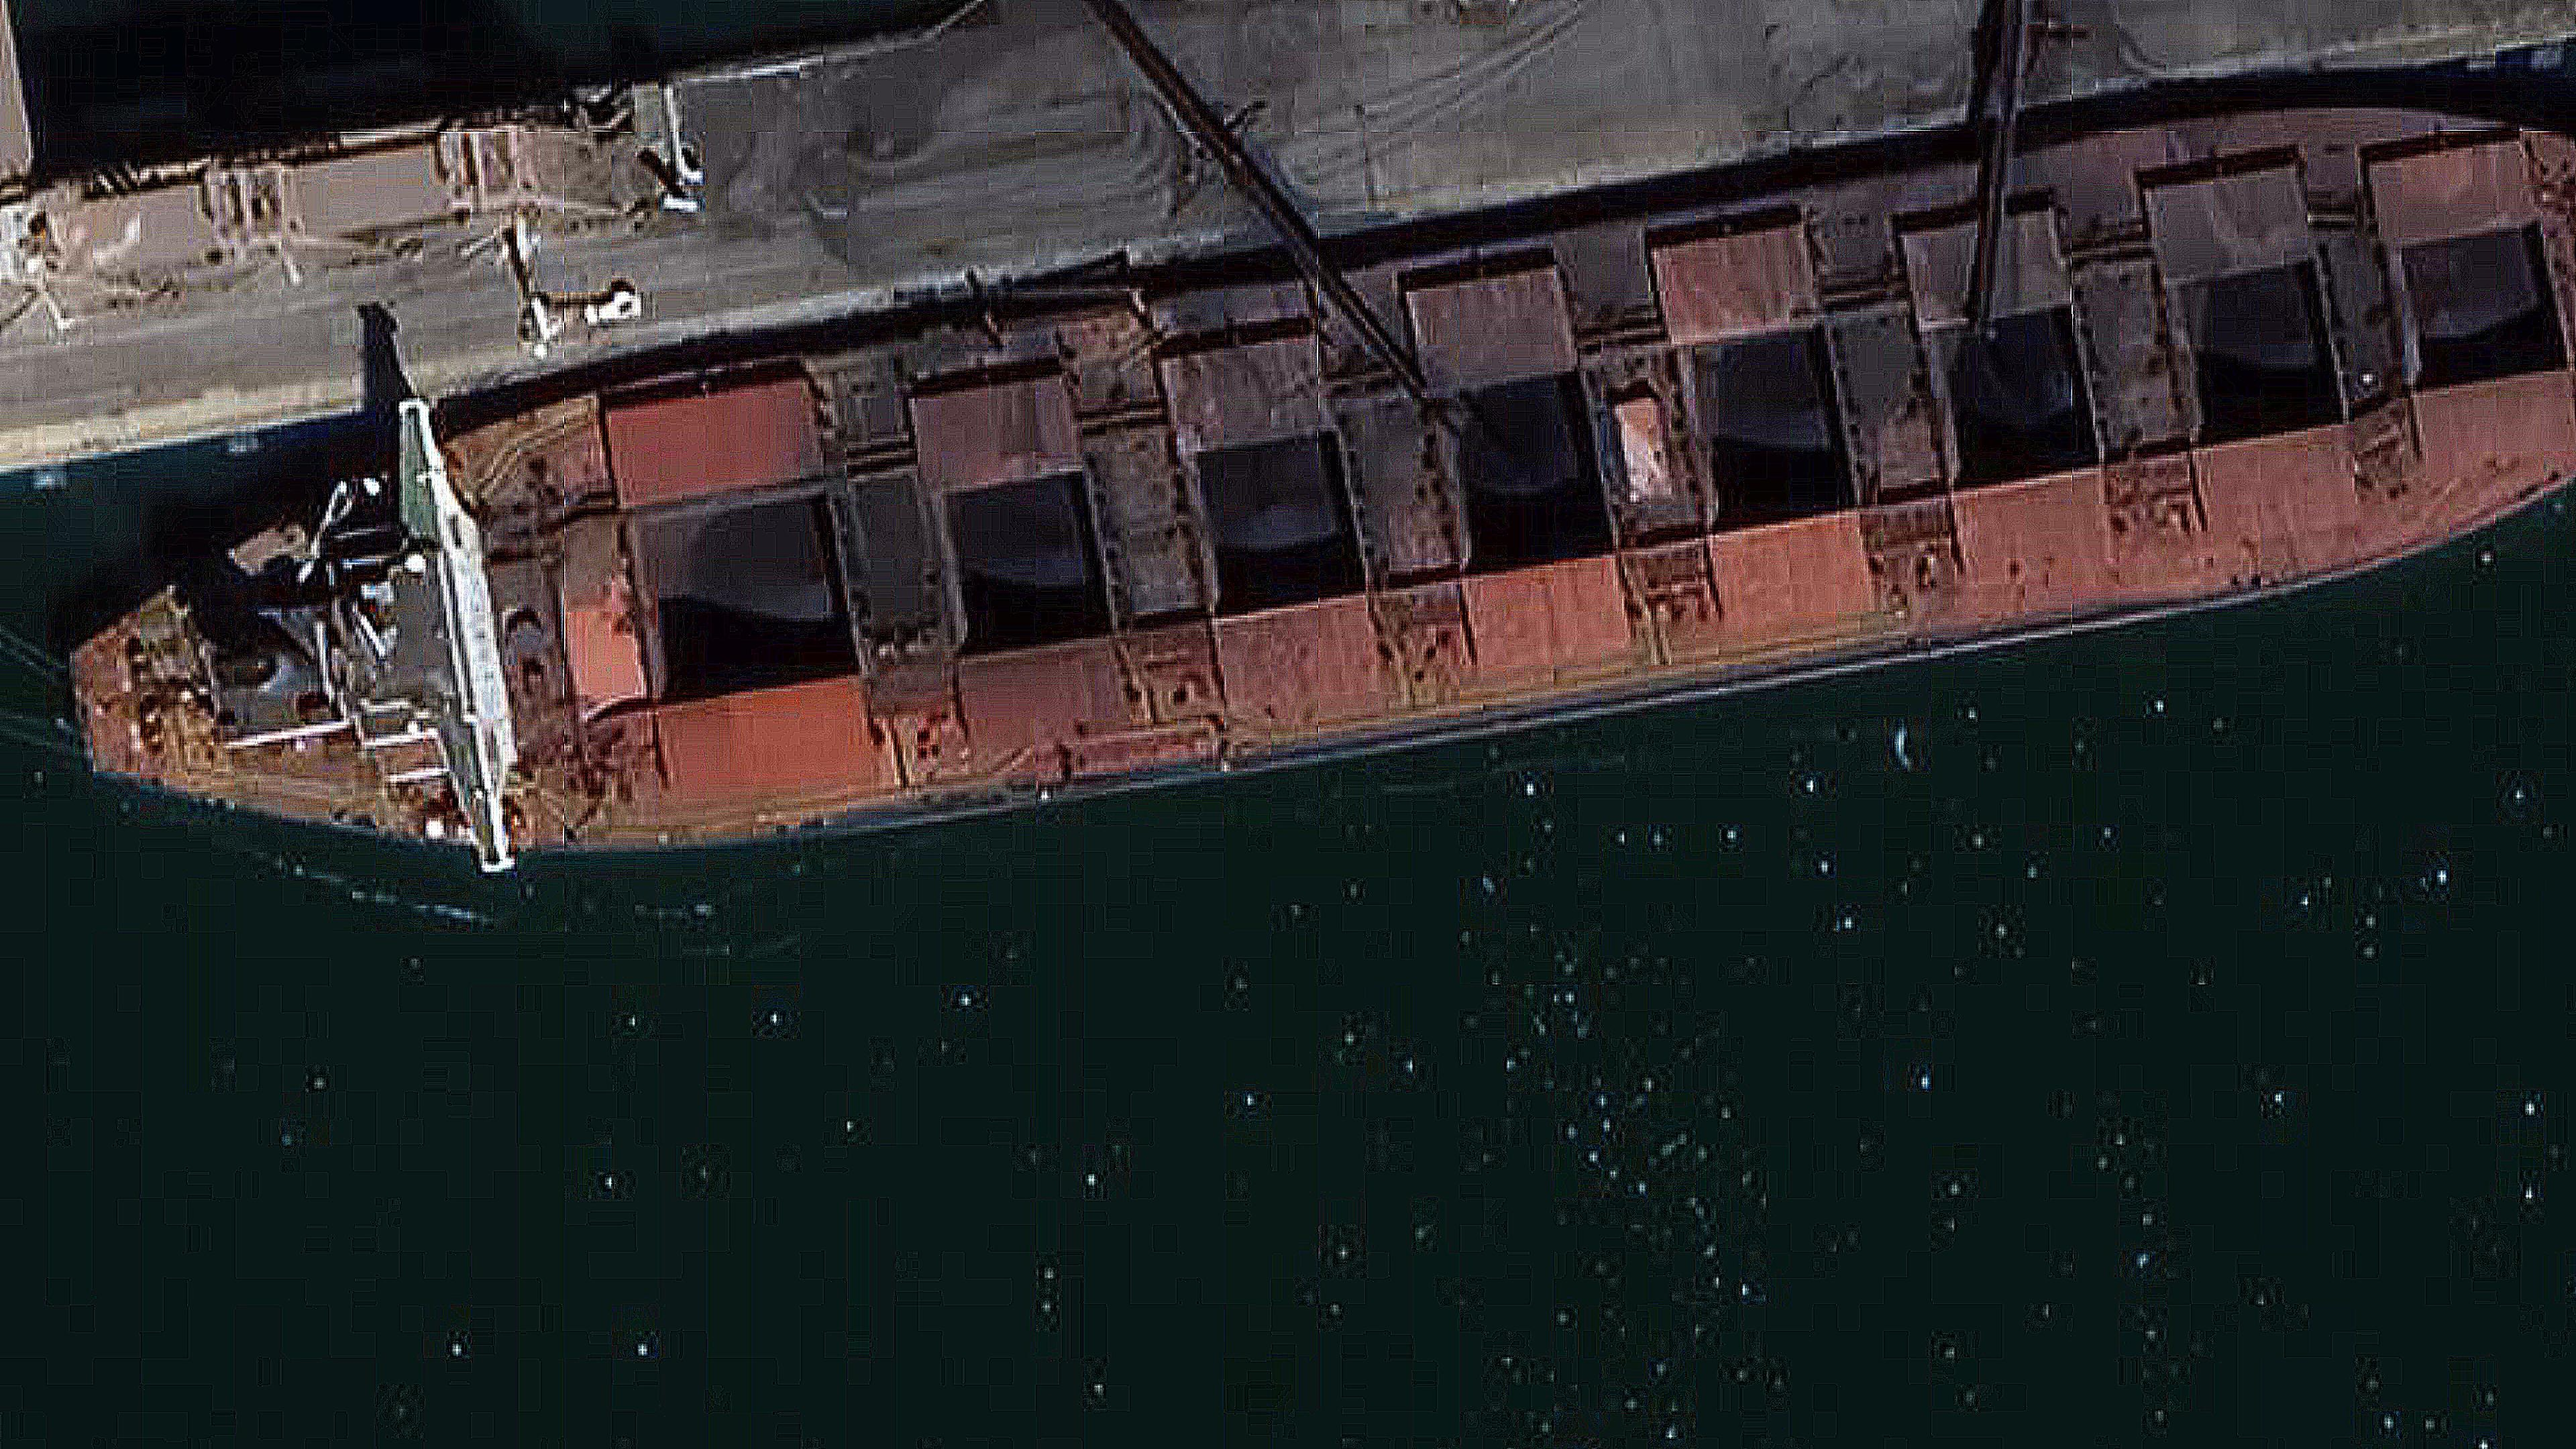
\includegraphics[scale=0.11]{img/Guaymas_202103_overflow_screen.jpg}
    \caption{A cargo (March 2021, Guaymas) overflowed the image and will be excluded from the statistics.}
    \label{fig:Guaymas_202103_overflow_screen}
\end{figure}


\begin{figure}
    \centering
    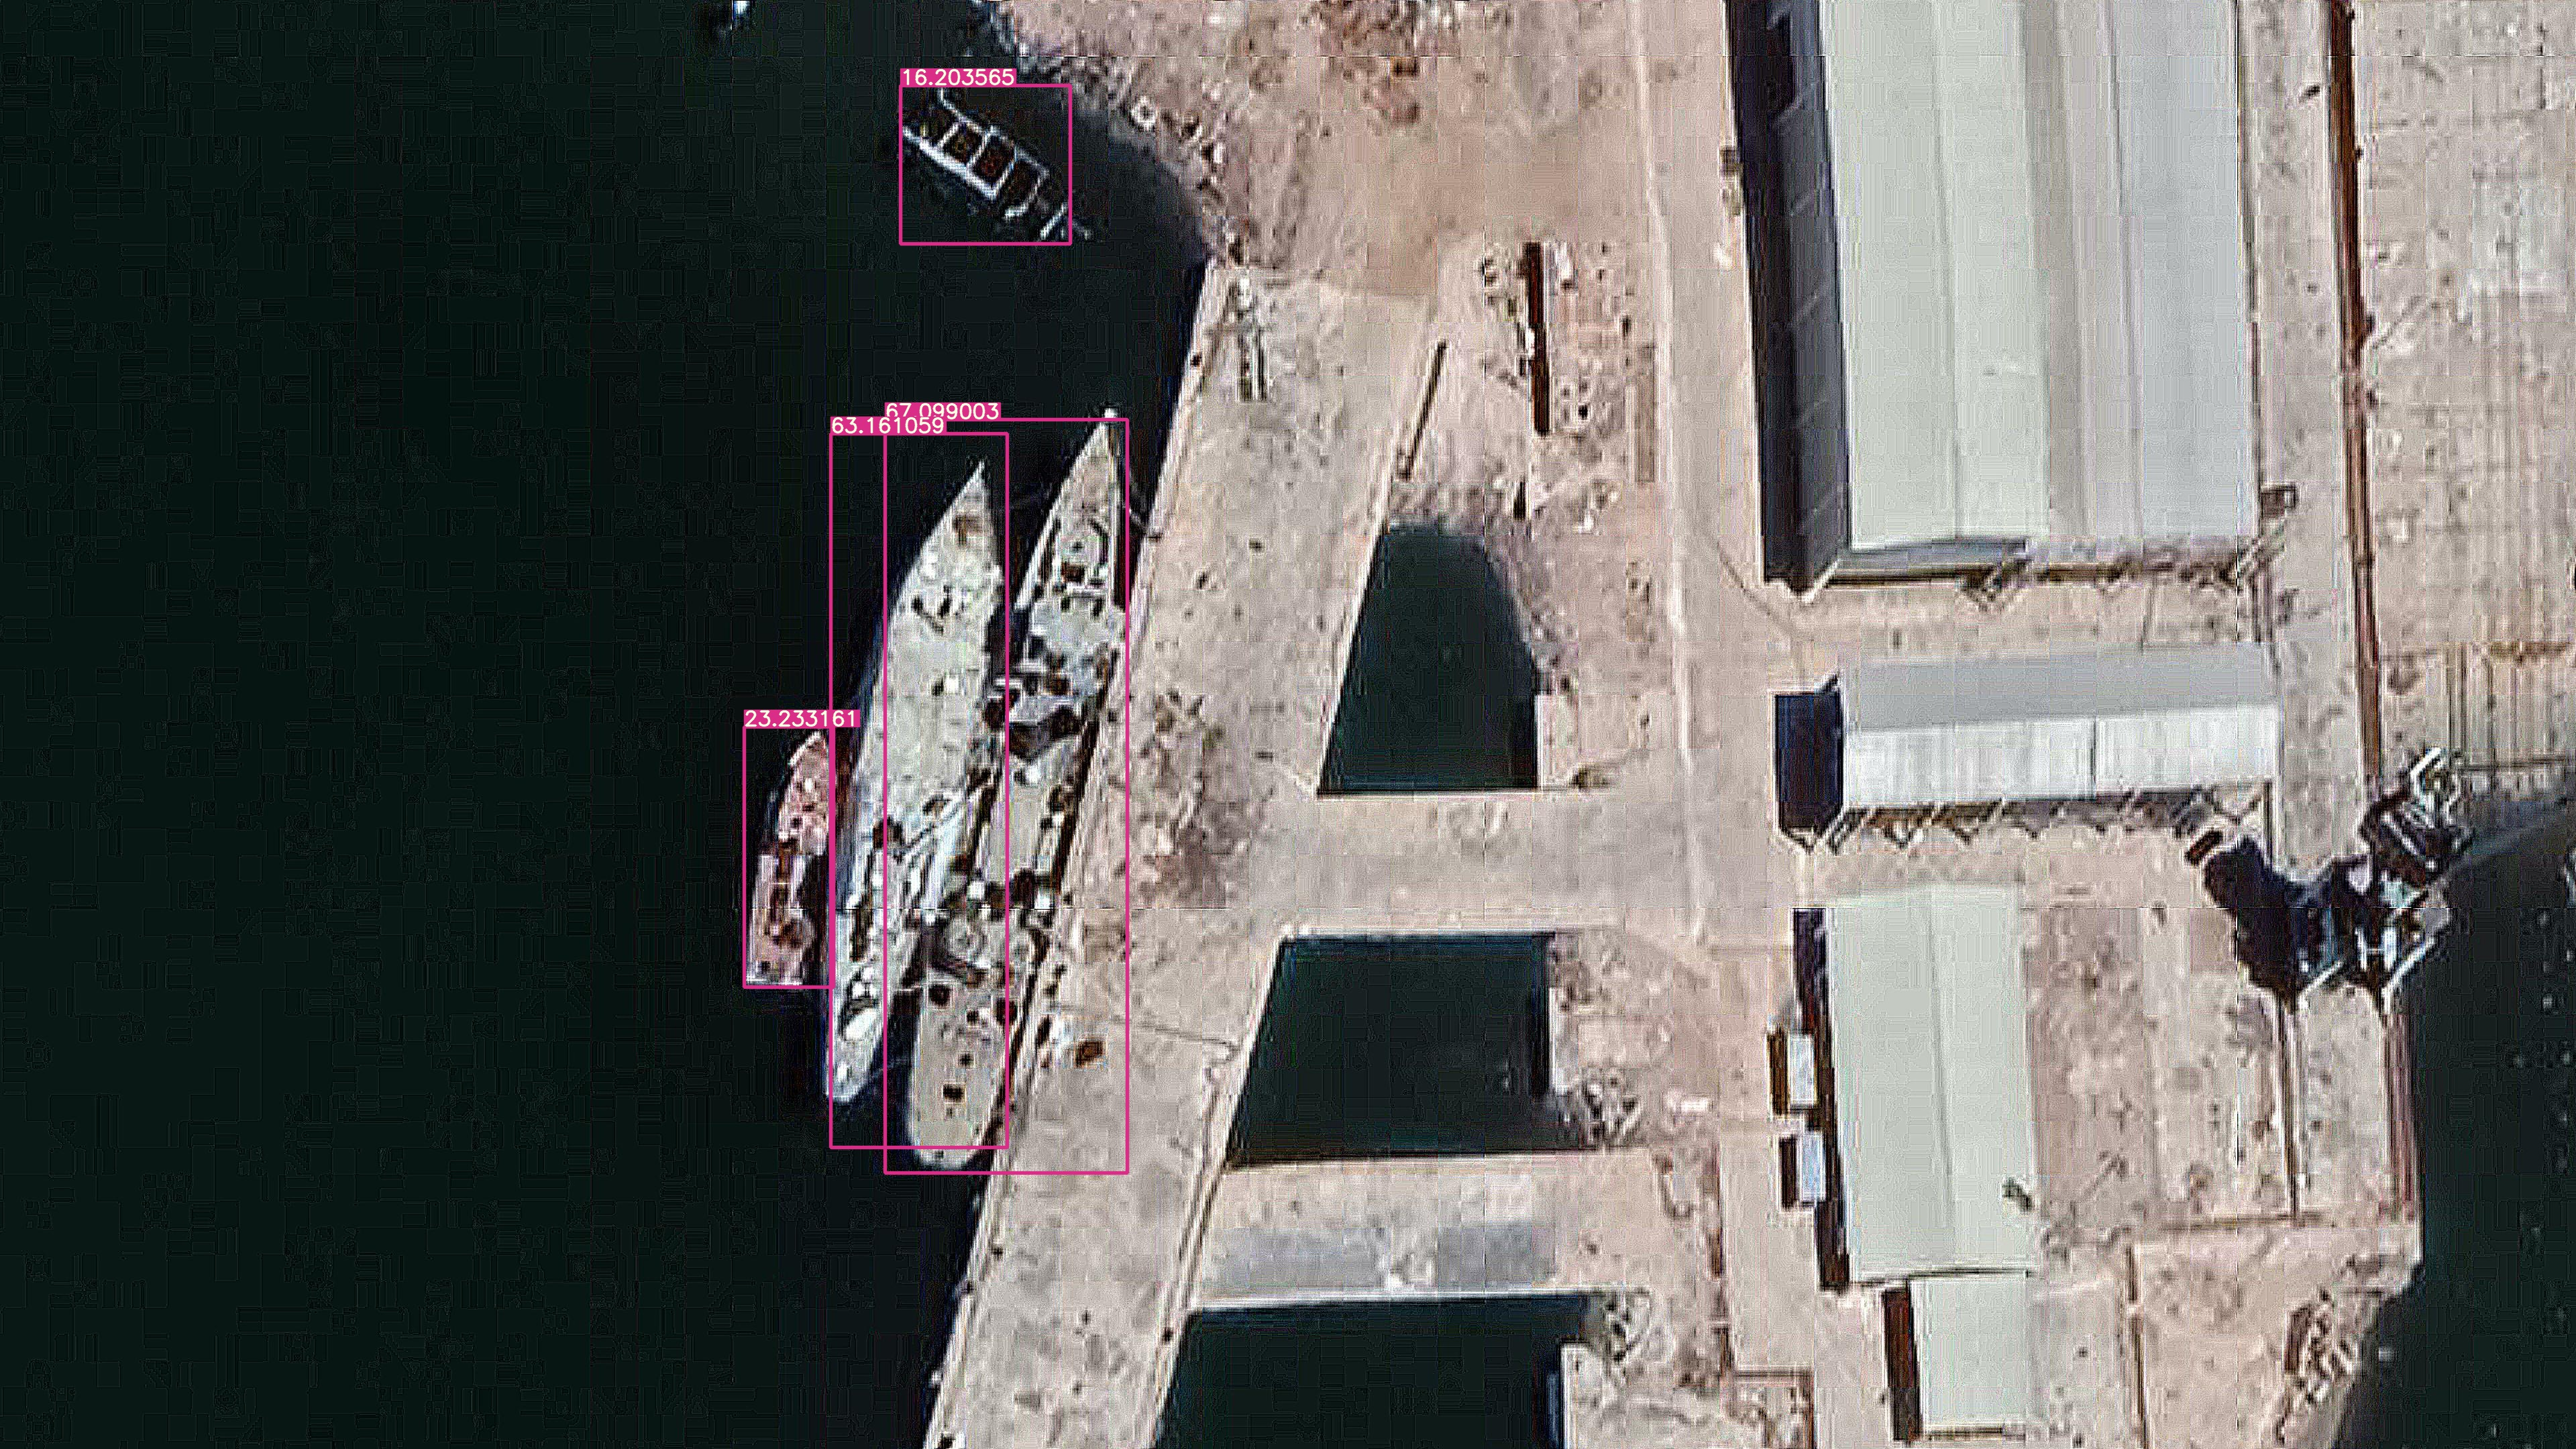
\includegraphics[scale=0.11]{img/Guaymas_202105_detect_small_large.jpg}
    \caption{The algorithm can detect all the boats (May 2021, Guaymas) well if no big boats overflowed the image.}
    \label{fig:Guaymas_202105_detect_small_large}
\end{figure}




\subsection{Classification of Entertainment Boats and Fishing Boats}
\label{sec:3.2.5}
After distinguishing between large and small boats, it is necessary to distinguish between small recreational boats for domestic use and fishing boats without a roof. In this thesis, whether or not the colour shown on satellite images of detected small boats is mostly white becomes a feature that distinguishes recreational boats from fishing boats. To do this, we need to find the range of small boats previously identified by the algorithm, i.e. the four coordinates of the anchor box. Then, analyse whether the colour within the anchor frame is white or close to white. Finally, the number of white boats is counted.


\section{Workflow}
The flow chart from the training data to the final statistics made is shown in Figure~\ref{fig:workflow}.
\begin{figure}[h]
    \centering
    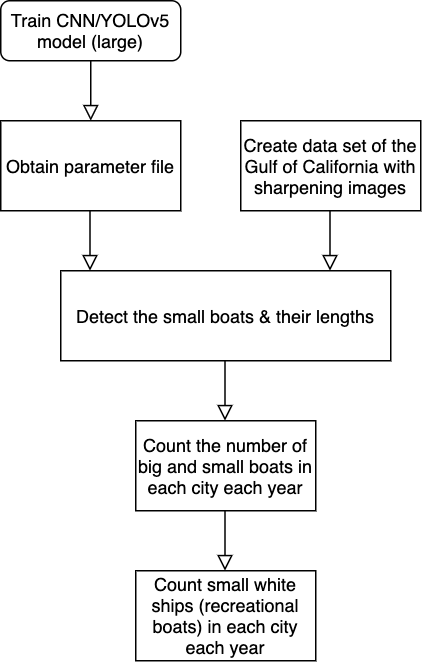
\includegraphics[scale=0.6]{img/workflow.png}
    \caption{The workflow of detection.}
    \label{fig:workflow}
\end{figure}


% Results
\chapter{Results}
\label{chapter:Results}

\section{Train Custom Data}
\subsection{Weights and Biases Logging}
\subsection{Local Logging}
\subsection{The Best Weight and Testing Results}

\section{Detection and Classification}

\section{Differences in Vessel Composition in Santa Rosalia, Loreto, Guaymas}

% Conclusion
\chapter{Conclusions and Future Work}
\label{chapter:Conclusions_and_Future_Work}
 % 1. Draw together all the work and results in the above report and to present a succinct summary.
 \section{Draw together all the work and results}
 
 % 2.Future Work: 本来应该分类成「更加精确的分类」Leisure boat / Shipping boat / family boat... 需要更多清晰 (分辨率 + 颜色) 的测试数据集... 在训练数据的时候就很清晰要分类成什么.....) + 扩展到更多的地区
 \section{Future Work}
 
 % 3. 画大饼 propose
\section{Pathway + Propose}
 
 % 4. Include a brief reflection on what I have learnt from undertaking my project as far as project management is concerned.
 
\section{Brief Reflection}

% Bibliography
\bibliographystyle{bartlett_harvard_ref}
\bibliography{ref}

\end{document}
